Distributed ledger technology (DLT) is a data structure distributed across multiple managing stakeholders. A subset of DLT is blockchain, which is a less efficient, immutable data structure with a slightly different trust model. Rauchs et al. of the Cambridge Centre for Alternative Finance provide a detailed taxonomy and conceptual framework \cite{rauchs2018distributed}. It can be seen in their paper that the definitions are somewhat unclear in literature.\par
DLT, and especially blockchain, are rapidly gaining ground in the public imagination, within financial technology companies (FinTech), and in the broader corporate world. \par
The technology and the global legislative response are somewhat immature, and misapplications of both technologies are commonplace. \par
Distributed trust models emerged from cryptography research in the 1970s when Merkle, Diffie, and Hellman at Stanford worked out how to \href{https://medium.com/swlh/understanding-ec-diffie-hellman-9c07be338d4a}{send messages online} without a trusted third party \cite{diffie1976new,merkle1978secure}.\par
Soon after the 1980s saw the emergence of the cypherpunk activist movement, as a reaction to the emerging surveillance state \cite{burnham1983rise, chaum1985security}, a topic which is expanded for this moment in a later chapter. These early computer scientists in the USA saw the intersectionality between information, computation, economics, and personal freedom \cite{lavoie1990prefatory}. Online discussion in the early nineties foresaw the emergence of trans-national digital markets, what would become the WWW \cite{salinCosts, cypherPunkMailList}. The issues of privacy %(https://nakamotoinstitute.org/static/docs/cypherpunk-manifesto.txt) 
 and the exchange of digital value (digital / ecash) %(https://www.wired.com/1994/12/emoney/  https://www.cs.ru.nl/~jhh/pub/secsem/chaum1985bigbrother.pdf) 
 were of foremost importance within these discussions %(https://www.wired.com/1994/12/emoney/), 
 and while privacy was within reach thanks to \href{https://www.openpgp.org/about/history/}{``public/private key pairs''}, 
 ecash proved to be a more difficult problem. \par
Adam Back's 1997 `hashcash' \cite{back2002hashcash} paved the way for later work by implementing the concept of what would become `proof of work' \cite{dwork1992pricing, jakobsson1999proofs}. This was built upon by Dai \cite{dai1998b}, Szabo \cite{szabo1997formalizing}, Finney \cite{callas1998openpgp}, and Nakamoto amongst others. In all it took 16 years of collaboration on the mailing lists (and dozens of failed attempts) to attack the problem of trust-minimised, distributed, digital cash. The culmination of these attempts was Bitcoin \cite{Nakamoto2008}. This is illustrated by Dan Held in Figure \ref{fig:prehistory}. This is now a wider ecosystem of technologies and societal challenges (Figure \ref{fig:bitcointopics}). 

\begin{figure}
  \centering
    \includegraphics[width=\linewidth]{prehistory}
  \caption{Dan Held: \href{https://www.danheld.com/blog/2019/1/6/planting-bitcoinsoil-34}{Bitcoin prehistory} used with permission.}
  \label{fig:prehistory}
\end{figure}

\begin{figure}
  \centering
    \includegraphics[width=\linewidth]{bitcointopics}
  \caption{\href{https://twitter.com/djvalerieblove/status/1514703620272394243/photo/1}{Bitcoin Topics} used with permission @djvalerieblove.}
  \label{fig:bitcointopics}
\end{figure}

There is enormous complexity and scope, as seen in Figure \ref{fig:venn}, and yet genuinely useful products are elusive.
\begin{figure*}[ht]\centering % Using \begin{figure*} makes the figure take up the entire width of the page
	\includegraphics[width=\linewidth]{venn}
	\caption{\href{https://unchained.com/blog/blockchain-spectrum/}{Intersecting disciplines}. Reused with permission \href{https://unchained.com/}{Dhruv Bansal}}
	\label{fig:venn}
\end{figure*}
It is surprisingly hard to pin down a simple explanation for the features which define a blockchain. These ``key takeaway'' \href{https://www.investopedia.com/terms/b/blockchain.asp}{from Investopedia} are a neat summary however.\par
\textit{\begin{itemize} \item Blockchain is a specific type of database. \item It differs from a typical database in the way it stores information; blockchains store data in blocks that are then chained together. \item As new data comes in it is entered into a fresh block. Once the block is \href{https://bits.monospace.live/}{filled with data} it is chained onto the previous block, which makes the data chained together in chronological order. \item Different types of information can be stored on a blockchain but the most common use so far has been as a ledger for transactions. \item In Bitcoin’s case, blockchain is used in a decentralized way so that no single person or group has control—rather, all users collectively retain control. \item Decentralized blockchains are ``append only''. In effect this means that the data entered becomes irreversible over time. For Bitcoin, this means that simple economic transactions are permanently recorded and viewable to anyone. \end{itemize}}
In principle blockchains provide a \textbf{differentiated trust model}. With a properly distributed system a blockchain can be considered ``trust-minimised'', though certainly not risk minimised. This is important for some, but not all people. There is not much emboldening of text within this book. If you start to question the whole reason for this `global technology revolution' then it always comes back to those three words. \par
It can in fact be argued that the whole concept of distributed cryptographic blockchains is \href{https://www.trailofbits.com/reports/Unintended_Centralities_in_Distributed_Ledgers.pdf}{somewhat strained}, as the vast majority of the technology offerings are not distributed, and worse, meaningful distribution may indeed be practically impossible without a trusted third party \cite{kwon2019impossibility}. ``There are many scenarios where \href{https://calpaterson.com/blockchain.html}{traditional databases} should be used instead''\cite{casino2019systematic}.\par
\section{What's this for sorry?}
The proponents of blockchains argue, that in an era when data breaches and corporate financial insolvency intersect with a collapse in trust of institutions, it is perhaps useful to have an alternative model for storage of data, and value. That seems like a lot of effort for a questionable gain. It's far more likely it's simply speculation.\par 
While writing this book the questions of `what is this \textit{really for} and how can it possibly be worth it', came up again and again. In truth it's a very difficult question, without a clear enough answer. It's beyond the scope of this book to figure this out properly, but references to advantages and disadvantages will be made throughout.\par  
It seems that the engineers who created Bitcoin wanted very much to solve a technical problem they saw with money (from their understanding of it), and the transmission of money digitally. As the scale and scope have increased so has the \href{https://medium.com/@nic__carter/visions-of-bitcoin-4b7b7cbcd24c}{narrative evolved} as seen in Figure \ref{fig:Evolving}, but it's never really kept pace with the level of the questions posed. \par
\begin{figure*}[ht]\centering % Using 
	\includegraphics[width=\linewidth]{evolvingnarrative}
	\caption{The narrative use of Bitcoin has evolved, by Nic Carter and Hasufly.}
	\label{fig:Evolving}
\end{figure*}
A cost benefit analysis that excludes speculative gains seems to fail for pretty much all of blockchain/DLT. Bitcoin is more subtle as it possibly \textit{can} circumvent the legacy financial systems. This still leaves huge questions. To quote others in the space, is Bitcoin now the iceberg or the life raft? \par 
For the most developed defence of the technology as it stands in from a Western perspective, in this moment, Gladstein (\href{https://www.financialinclusion.tech/}{and others}) offer a vision for the asset class, in the 87\% of the world he says don't have access to the technology infrastructure benefits enjoyed by the developed west \cite{gladsteincheck2022} (Figure \ref{fig:walledworld}). 
\begin{figure*}[ht]\centering % Using \begin{figure*} makes the figure take up the entire width of the page
	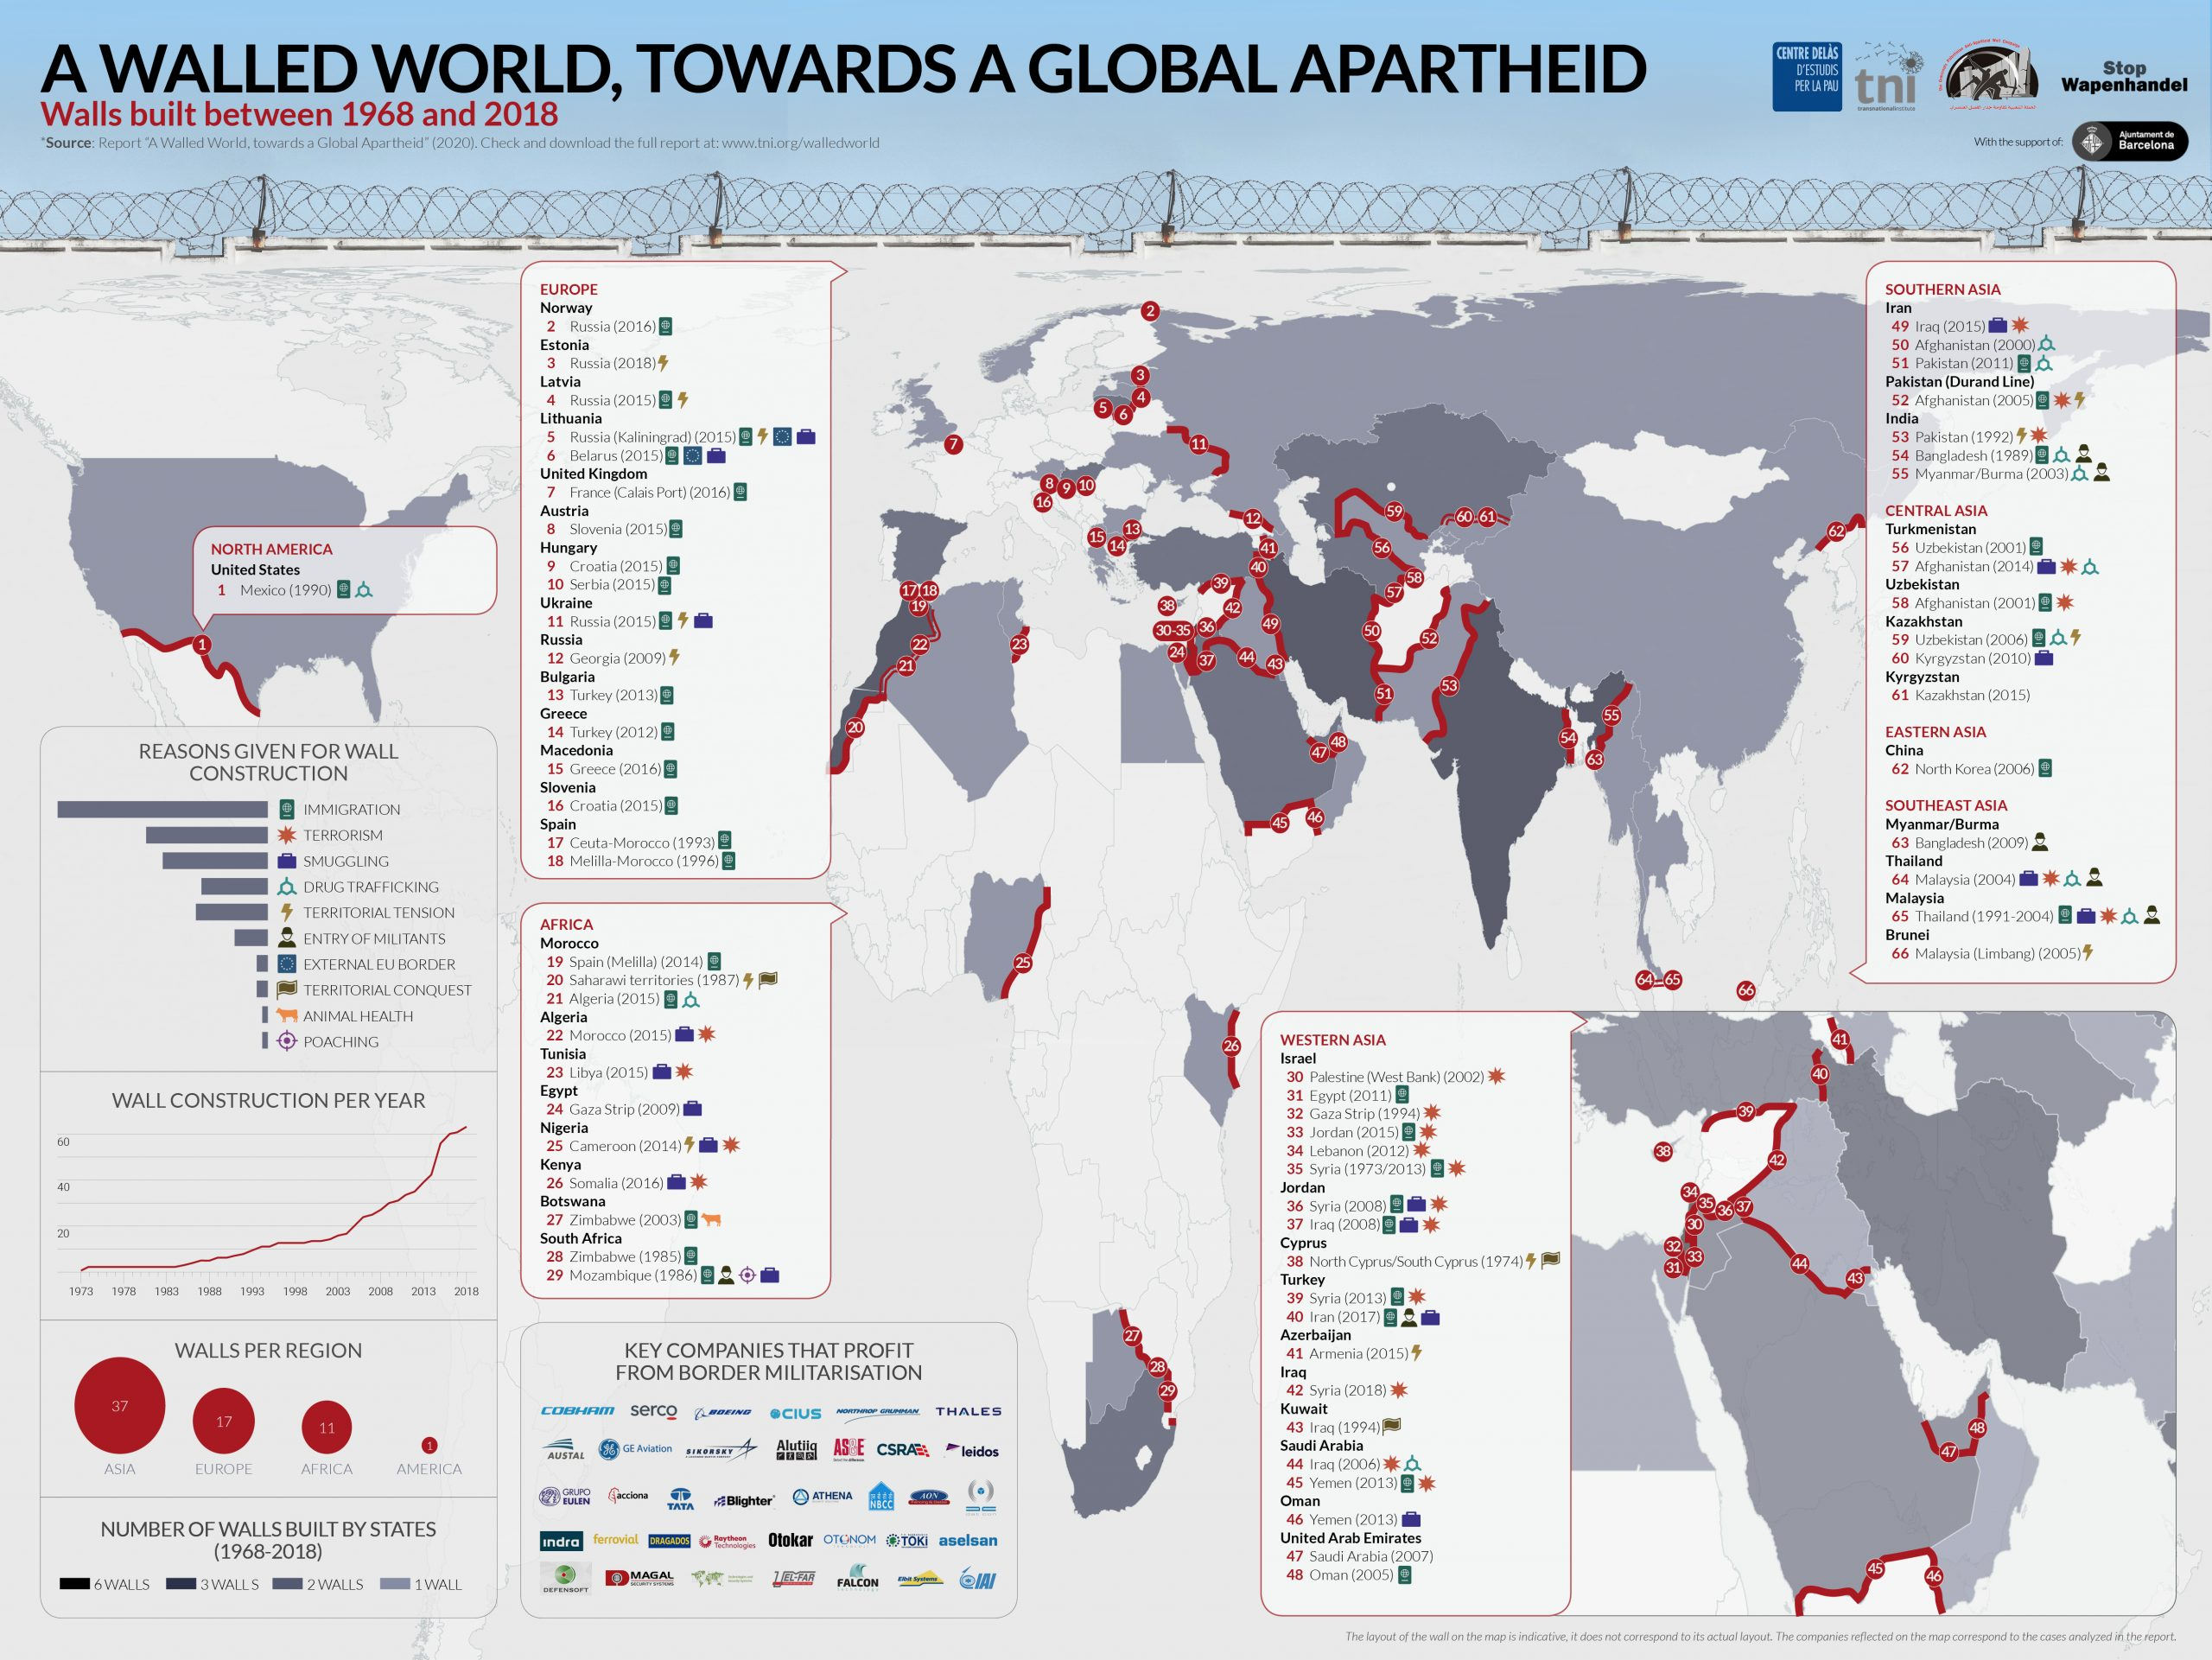
\includegraphics[width=\linewidth]{walledworld}
	\caption{We live in an increasingly \href{https://www.tni.org/en/walledworld}{walled world} (tni, rights requested)}
	\label{fig:walledworld}
\end{figure*}
He points to Block and Wakefield Research's report which finds those living under financially oppressive regimes are the most optimistic about the technology as in Figure \ref{fig:optimism}. This argument is suggestive of huge and untapped markets for services which may be accessible to developed nations through telepresence/metaverse interfaces, and which may increase equity of access to opportunity elsewhere. To put some figures against this:
\begin{itemize}
\item Nigeria has the highest number of crypto owners in the world in 2022 with 45\% of its population owning or using cryptocurrency.
\item Thailand occupies the second space with 44\% of its population reported to be using or owning cryptocurrency.
\item Turkey has 40\% of its population owning and using cryptocurrency in 2022, equal to over 33 million people.
\item Argentina occupies the fourth position with an ownership and usage rate of 35\% in 2022, representing almost 16 million people.
\item United Arab Emirates has 34\% of the population owning or using cryptocurrency in 2022, representing almost 10 million people.
\item Philippines is ranked sixth with a 29\% adoption rate.
\end{itemize}
\begin{figure*}[ht]\centering % Using \begin{figure*} makes the figure take up the entire width of the page
	\includegraphics[width=\linewidth]{optimism}
	\caption{\href{https://twitter.com/gladstein/status/1532054253673406464}{``This new chart from Block is financial privilege visualized.''}}
	\label{fig:optimism}
\end{figure*}
Gladstein's is a carefully developed and well researched book, but is \href{https://bitcoinmagazine.com/culture/imf-world-bank-repress-poor-countries}{written from the western perspective} of (just) Bitcoin `being the raft'. Later in this book we will consider if it might be the iceberg, but this is not the domain expertise we offer in this book. It is crucial to note that Gladstein has vociferous detractors within Africa. It seems entirely possible he's another grifter as suggested by Kimani: \textit{``Gladstein is a charlatan who makes his living by selling the image of a global south that is corrupt, entirely lacking in rational thinking and needing a saviour, like him to swoop in and save us from our floundering selves. He exploits on tired and unproven stereotypes, cherry picks data while ignoring mountains of evidence that disprove him. Because he knows that as the perceived ``morally superior'' ``right thinking'' western superior coming to save, he will mostly go unchallenged. It's a grift, an old grift that many like him have turned into an industry. Where they earn tax free income by selling a delusion and fetish to their western audience who need to think the global south is a failure of the human experience. He is trying to set himself up as some gate keeper and king maker in the Global South. He knows that the next phase of growth is. So he wants to make sure that westerners looking to invest in the global south  see him as some ``expert'' and ask for his unfounded opinions. People like him run global morality extortion rings. How so? Simple: By purporting to know and be the keeper of global south morality, he will use his words to bless or curse your business, well, unless you make a generous donation to his foundation. These are scare tactics employed by charlatans to run tax-evading PR entities, thinly veiled as ``human rights'' organisations. If you are not on his side, he will slander you and your organisation. If you ensure you promote him and his ambitions, he anoints you as the good guy! He is trying to play the role that the Vatican and other corrupt religious organisations played in the 1800. Turning morality into a commodity that can be purchased from his market place: We decide who is good and who is bad and who can do business and who can't. For a ``donation''. He is not the first and he will not be the last. It's a growing industry, driven by shrewd westerners who know that they can sell racial stereotypes back home, but as long as they claim they are the one's helping or saving the coloured peoples from themselves.''} \par
%To further contextualise this \href{https://www.youtube.com/watch?v=BRQIMjZLMDk}{Mike Novogratz} claims the adoption figures at the top of the page. 
\href{https://dailyhodl.com/2022/05/04/crypto-winter-unlikely-as-astonishing-user-growth-dwarfs-internet-adoption-rate-macro-guru-raoul-pal/}{Raoul Pal of RealVision} says: \textit{Crypto adoption is now massively outperforming the internet. It’s been growing at about 165\% a year versus 85\% for the internet for the same period of time now.} According to analytics company Chainalysis; growth is fastest in the Middle east and North Africa (Figure \ref{fig:grow}). \par
\begin{figure*}[ht]\centering % Using 
	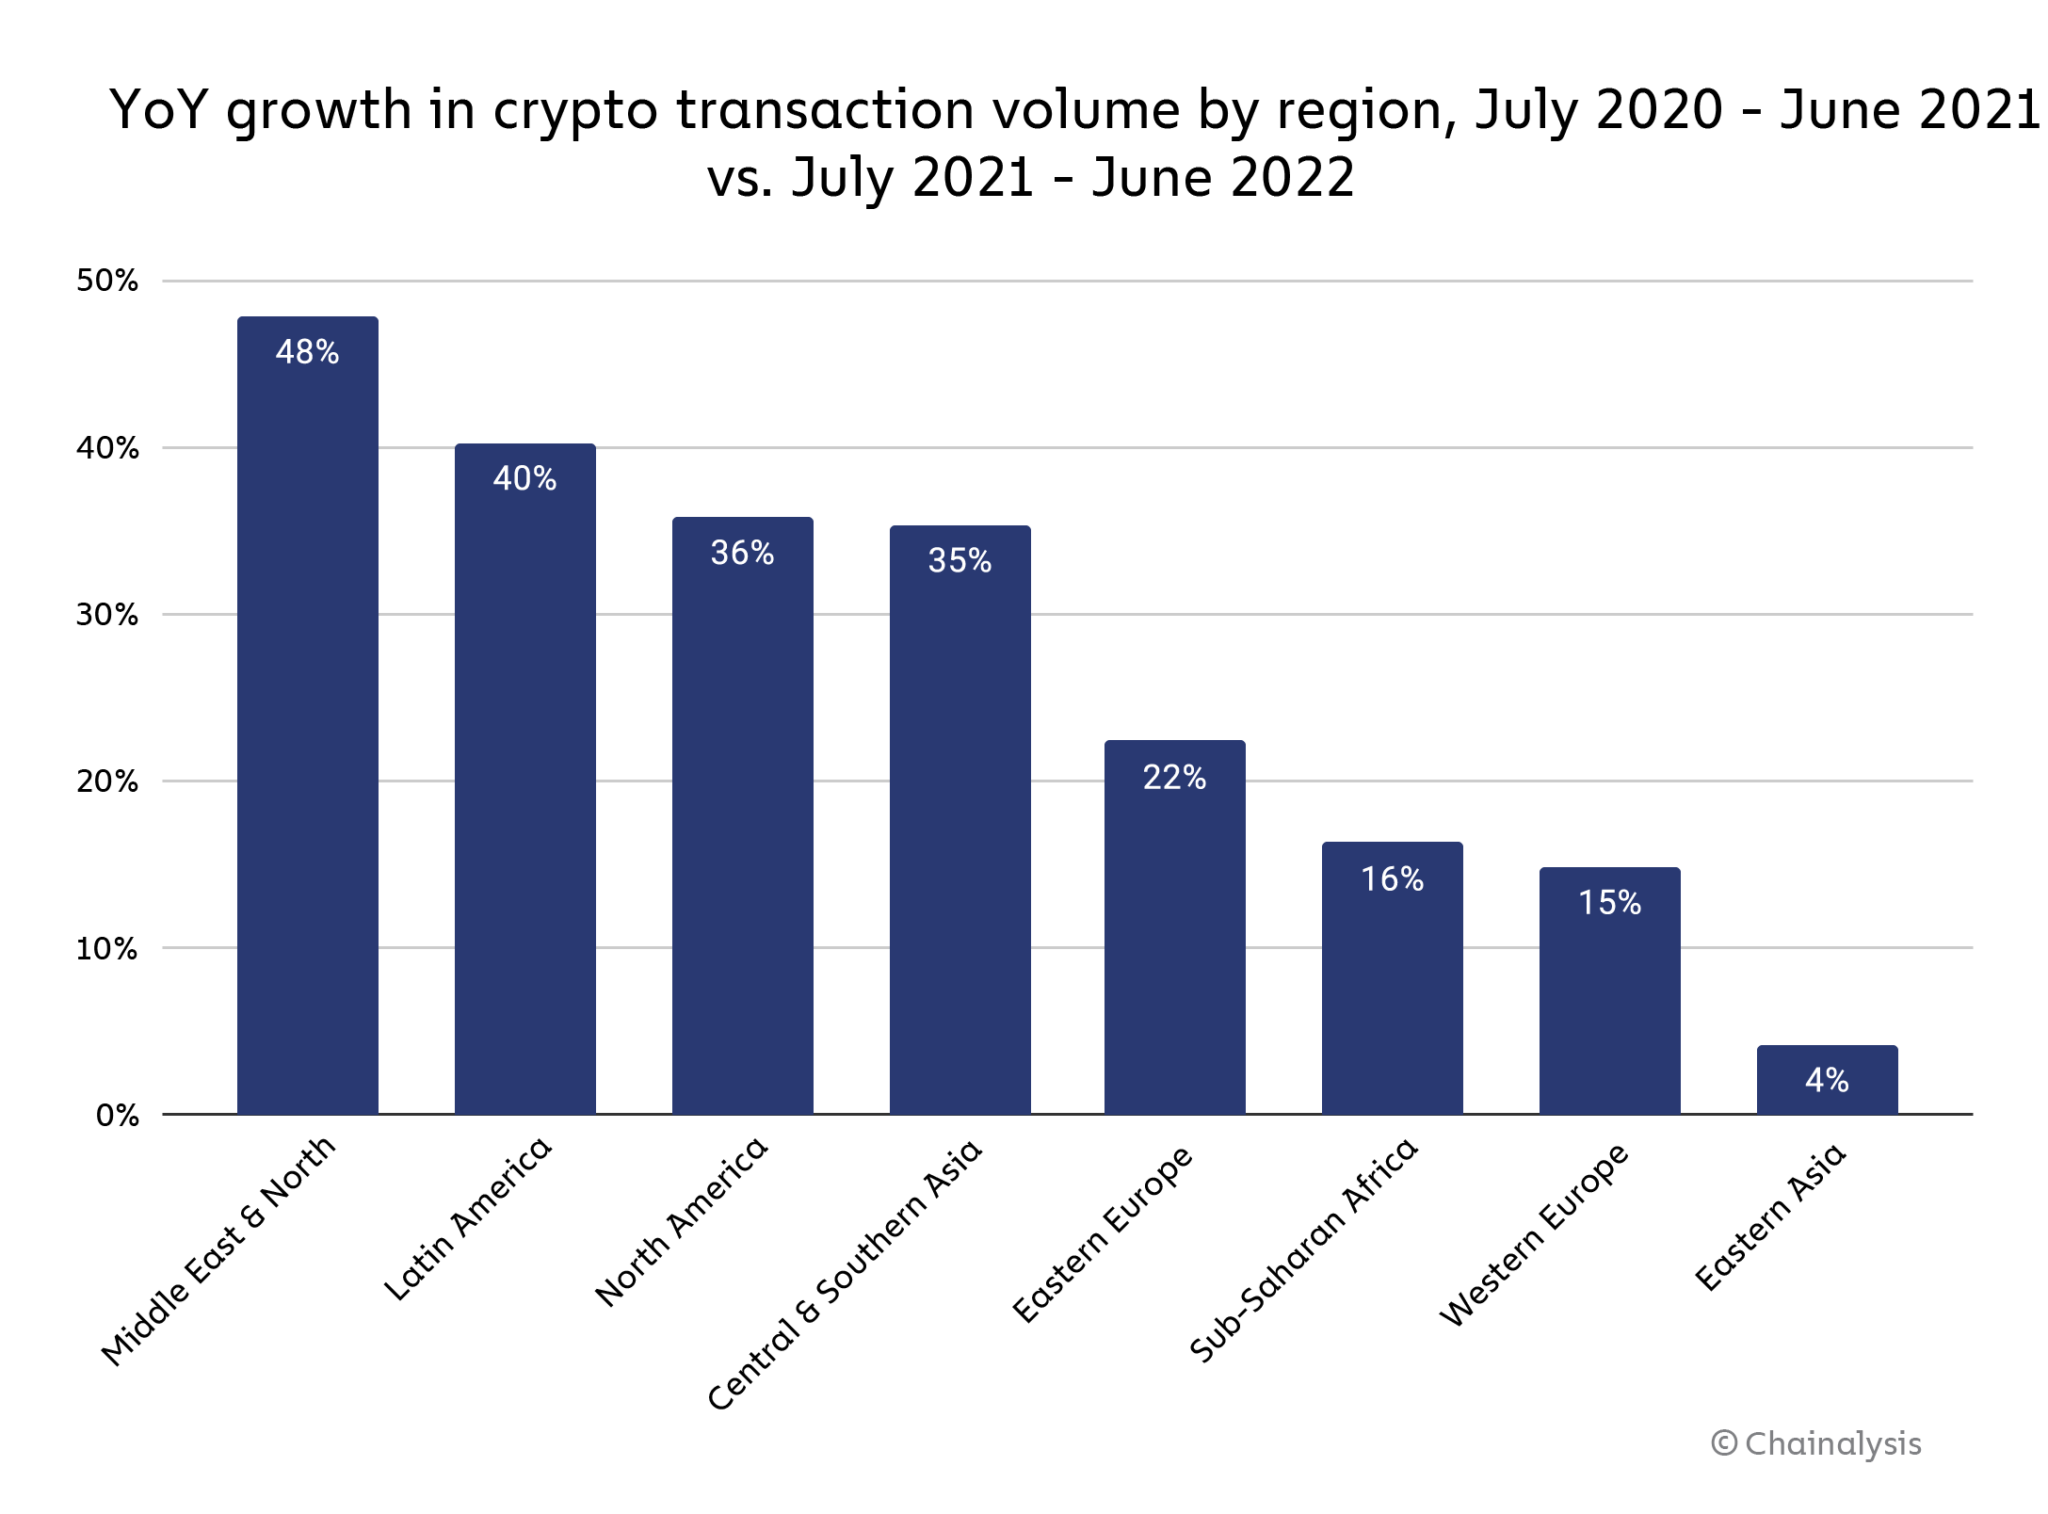
\includegraphics[width=\linewidth]{grow}
	\caption{Rapid growth is mainly outside of `Western Markets'}
	\label{fig:grow}
\end{figure*}
Thanks to a natural fit with strong encryption, and innate resistance to censorship by external parties, these systems do lend themselves well to `borderless' applications, and are somewhat resistant to global regulation (for good or ill). Given the rates of adoption seen in Figures \ref{fig:grow}, \ref{fig:ownership}, \ref{fig:userFigures}, and \ref{fig:euroInvest} it seems that this stuff is coming regardless of their usefulness to the developed world. If we are to take this as a given then we can perhaps logically infer that finding a use case for the technology is important, somewhat irrespective of other arguments. This provides us an opportunity to explore for metaverse applications, and this will be the focus.
\begin{figure*}[ht]\centering % Using 
	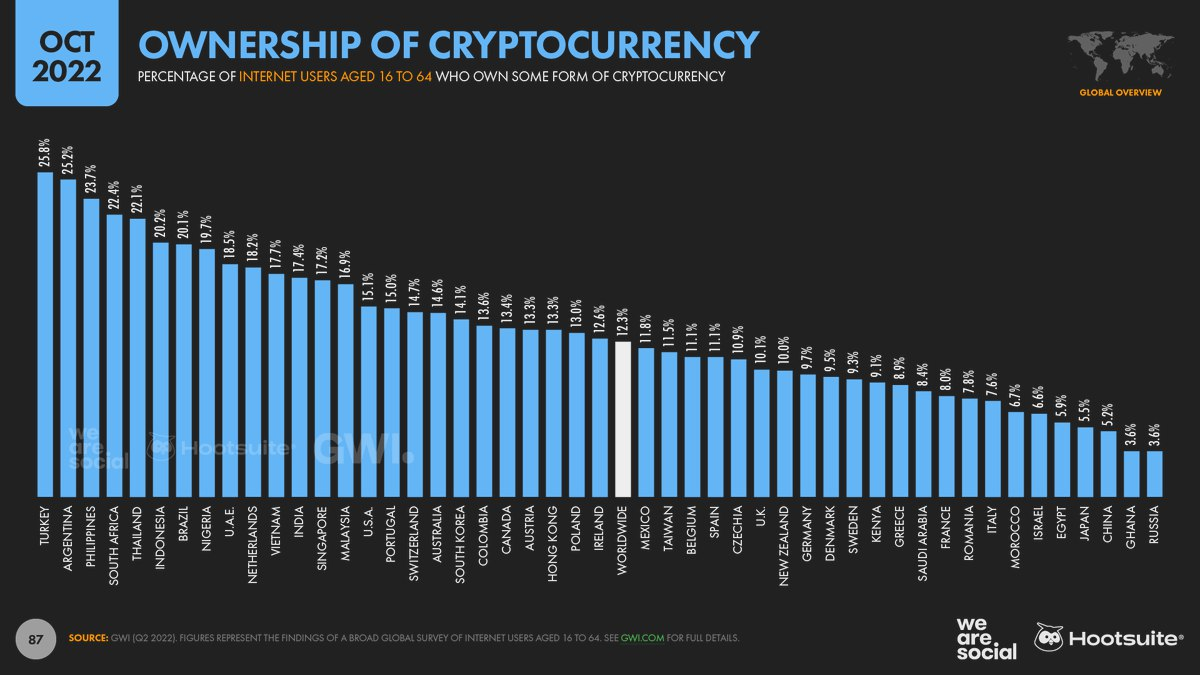
\includegraphics[width=\linewidth]{ownership}
	\caption{Rapid growth is mainly outside of `Western Markets' - 2}
	\label{fig:ownership}
\end{figure*}
\begin{figure*}[ht]\centering % Using 
	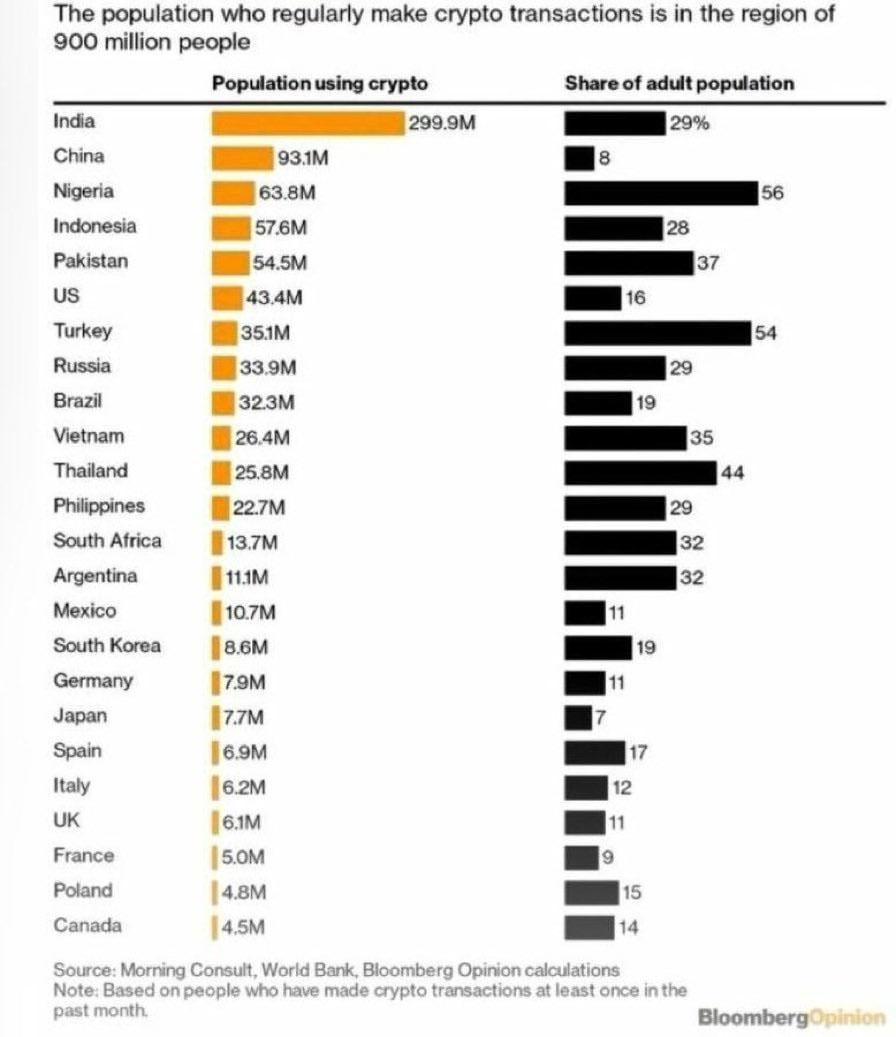
\includegraphics[width=\linewidth]{userFigures}
	\caption{Regular user numbers are surprisingly high.}
	\label{fig:userFigures}
\end{figure*}

\begin{figure*}[ht]\centering % Using 
	\includegraphics[width=\linewidth]{euroinvest}
	\caption{European crypto investment vs funds stocks and bonds from \href{https://github.com/gilbertfontana/DataVisualization}{Fontana} at \href{https://www.visualcapitalist.com/cp/crypto-popularity-in-europeans-union-nations/}{VisualCaptialist}}
	\label{fig:euroInvest}
\end{figure*}

%\begin{table}[]
\begin{tabular}{|l|r|l|r|}
\hline
\textbf{Country} & \textbf{\begin{tabular}[c]{@{}r@{}}\% of pop own\\ crypto\end{tabular}} & \textbf{Country} & \textbf{\begin{tabular}[c]{@{}r@{}}\% of pop own\\ crypto\end{tabular}} \\ \hline
Ukraine          & 12.7                                                                    & South Africa     & 7.1                                                                     \\ \hline
Russia           & 11.9                                                                    & Nigeria          & 6.3                                                                     \\ \hline
Venezuela        & 10.3                                                                    & Colombia         & 6.1                                                                     \\ \hline
Singapore        & 9.4                                                                     & Vietnam          & 6.1                                                                     \\ \hline
Kenya            & 8.5                                                                     & Thailand         & 5.2                                                                     \\ \hline
USA              & 8.3                                                                     & United Kingdom   & 5.0                                                                     \\ \hline
India            & 7.3                                                                     & Brazil           & 4.9                                                                     \\ \hline
\end{tabular}
\end{table}

\section{A panoply of tech}
Within DLT/blockchain there seem to be as many opinions on the value of the technology as there are implementations. A host of well engineered open source code repositories makes the cost of adoption relatively low. \par%Unfortunately there are many more repositories that look very similar and essentially scams.\par
There are thousands of different `chains' and many more tokens which represent value on them. A majority of these are code forks of earlier projects. Most \href{https://99bitcoins.com/deadcoins/}{are defunct} yet still have some residual `value' locked up in them as a function of their `distributed' tokens. \par 
Because the space is comparatively new, subject to \href{https://www.esma.europa.eu/press-news/consultations/call-evidence-dlt-pilot-regime}{scant regulation}, and often open source, it is possible to clone a github, change a few lines of code, and front it with a website in order to create `scams', and this happens frequently \cite{golumbia2020cryptocurrency}.\par
%An earlier version of this book talked about the opportunities and challenged with the dominant ``smart chain'' network; Ethereum. These pages can be \href{https://raw.githubusercontent.com/flossverse/product/draft/Book/03_ether.tex}{found in the github}, but were removed to improve the focus of this design. Now that Ethereum has transitioned to a more energy efficient consensus model our choice to dismiss the technology has become even more clear, and this will be explained later in the section.
The following sections give an overview of the major strands of the technology. First is Ethereum, mainly to discount it's use for our needs, and move on to more appealing options.

\section{Ethereum}
Ethereum \cite{buterin2013ethereum} is the second most \href{https://www.crypto51.app/}{secure} public blockchain (\href{https://howmanyconfs.com/}{by about 50\%})\cite{sayeed2019assessing}, and second most valuable by \href{https://coinmarketcap.com/}{market capitalisation} (though this comparison is somewhat stretched). It is the natural connection from Web3 to the rest of the book, so it will be considered first.\par
It is touted as `programmable money'. It, unlike bitcoin, is (\href{https://hackernoon.com/turing-completeness-and-the-ethereum-blockchain-c5a93b865c1a}{nearly}) Turing complete \cite{petzold2008annotated}, able to run a \href{https://ethereum.org/en/developers/docs/evm/}{virtual machine} within the distributed network (albeit slowly), and can therefore process complex transactional contracts in the settlement of value. This has given rise to the new field of `distributed finance', or DeFi (described later), alongside many interesting trust-minimised immutable ledger public database ideas. \par
There are trade-offs and problems with Ethereum (Eth/Ether) which currently increase the `participation floor' and make the network far less suitable for entry level business-to-business use. The ledger itself being a computational engine, with write only properties, is enormous. Specialist cloud hardware is required to run a full node (copy of the ledger), and partial nodes are the norm. Many partial nodes are run by one specialist cloud provider (\href{https://consensys.net/blog/news/why-infura-is-the-secret-weapon-of-ethereum-infrastructure/}{Infura}), which has recently been forced to \href{https://finance.yahoo.com/news/metamask-infura-block-certain-areas-173749914.html}{exclude Venezuela} from the network. Network validators are \href{https://mevwatch.info}{refusing to process} addresses on an \href{https://home.treasury.gov/policy-issues/office-of-foreign-assets-control-sanctions-programs-and-information}{OFAC sanction list}. A staggering 58\% runs on \href{https://ethernodes.org/networkType/Hosting}{Amazon AWS servers}. Critics of the project point to these vulnerabilities to outside influence as an existential threat to the aims of the technology. If it can be censured, then what advantage is there over the \href{https://protos.com/consensys-lawsuit-jpmorgan-owns-critical-ethereum-infrastructure/}{founders} simply running a high speed database to the same purpose? \par
This is a function of the so called `scalability trilema' \cite{hafid2020scaling}, in which it seems that only two features from the list of decentralization, scalability or security can be chosen for blockchains \cite{bonneau2015sok}.\par
Moreover the network is \href{https://bitcoinmagazine.com/technical/ethereum-is-coercive-bitcoin-is-not}{centrally controlled} by its creator and the `miners'. There is a strong case to answer that Eth is \href{https://blog.mollywhite.net/blockchains-are-not-what-they-say/}{neither distributed}, nor trustless, and in fact therefore fails to be differentiated from a DLT, undermining some of it's claims. The history of Ethereum is a fascinating case study in human greed. By the time the whitepaper had it's first limited release, Bitcoin (covered next) had already passed \$1000 per token. This led to the creators ambitions for a `fair release' of tokens being voted down by powerful funders, leading to the explosion of similarly structured `pre-mined' coins in the ICO craze, which followed on the Ethereum network. Laura Shin is possibly the most experienced journalist and author in the space and has covered this crazy era in her book `The Cryptopians' \cite{cryptopians}. It's a tough read for the newcomer though, perhaps finish this primer first!\par
With that said there are many talented developers doing interesting work on the platform, and innovation is fast paced. It is entirely normal for technology projects to launch their distributed ledger idea on and within the Ethereum network. These generate tradable `ERC-20' tokens, which can accrue value or demonstrate smart contract utility  (based on the \href{https://soliditylang.org/}{Solidity} programming language). Because the value locked and generated in the Ethereum platform comes not just from the ETH token, but all the ERC technologies built upon it, there are hundreds of billions of pounds `within' the network. All of these projects, and indeed the core technology of Ethereum are subject to exploits and vulnerabilities and tens of billions of pounds have been lost \cite{chen2020survey}. Most of this money is pure market speculation (as is the case across blockchains). Many analysts cannot see this as anything but a speculative bubble, with all the predictable crash yet to come. This can be seen in the context of other bubbles in Figure \ref{fig:etherbubble}. It seems that most of the projects in crypto more generally, but certainly with ETH and the NFTs within it are a new kind of social gambling, where online communities can reinforce groupthink around their speculative choices. This idea that Ethereum is not a commodity, but rather a security, built around promises of returns, is finding recent favour in law. New York attorney general James has alleged that Ether is a security in \href{https://www.docdroid.net/Myyp0yz/kucoin-pdf#page=11}{court proceedings}, which could have enormous consequences, potentially reversing the momentum the asset had been enjoying as a commodity.   Jason Lowery of MIT and US Space Force \href{https://twitter.com/JasonPLowery/status/1572275617344757760}{lays out} a very clear thesis on the difference between Natamoto consensus and most of what followed as part of his PhD \cite{Lowery2023}. His explanation here is one of the reasons why we focus on Bitcoin, and dismiss `proof of stake' models: \par
\textit{``The innovation behind PoW is precisely the fact that it \textbf{doesn't} rely exclusively on software (an abstraction) to keep the ledger systemically secure, but instead incorporates real-world physics (watts) to impose real-world physical constraints on people/computers who run it. Stake is an abstraction. It is an imaginary way to describe the complex emergent behaviour of a bunch of general-purpose state machines. The state machines may physically exist, but the way you choose to visualize the complex emergent behaviour of those machines is imaginary. Satoshi didn't couple control authority over ledger to abstract, imaginary things like `stake' or `coin' precisely because these things don't physically exist. If they don't physically exist, they are incapable of imposing real-world physical costs on people seeking control of ledger. The real-world physical cost of controlling the ledger is what keeps control over the ledger decentralized. It is too physically expensive (in watts) to gain and maintain centralized control over the BTC ledger. In proof of stake, there is no physical cost of gaining centralized control. Why? Because stake doesn't physically exist. So all it takes to gain centralized control is majority stake. And once you have it (which, because of math, some combination of people already do), you have it forever.}


With all this said most of the \href{https://www.statista.com/statistics/1266322/nft-user-number/}{couple of million people} who have used NFTs use Ethereum, and if this market of creators and consumers is to be brought into a mixed reality space then they will need a way to bring their objects with them. 
\begin{figure}
  \centering
    \includegraphics[width=\linewidth]{etherbubble}
  \caption{Ethereum is thought to look like a speculative bubble. Rights requested}
    \label{fig:etherbubble}
\end{figure}
Such is the level of nefarious activity on these networks (within Ethereum) that they have a poor reputation, and are difficult to audit, launch, and maintain. The overriding problem of using a blockchain for utility applications (rather than just as money) is that people can, and will, simply lie for criminal purpose when entering data into the ledger. It is far more likely that Ethereum is simply a speculative bubble than any of the claims for utility being born out. Add to that \href{https://advisor.morganstanley.com/daron.edwards/documents/field/d/da/daron-edwards/Cryptocurrency_201__What_is_Ethereum_.pdf}{Morgan Stanleys recent assertion} that Ethereum is itself threatened by newer contender chains and it's future becomes unclear. The report correctly identifies that ``High transaction fees create scalability problems and threaten user demand. High costs make Ethereum too expensive for small-value transactions.''. It is this high cost of use that most excludes the ERC-20 networks from our consideration.
\subsection{Gas fees}
Ethereum has a significant barrier to entry because of high fees to use the network. The system is Turing complete; able to programatically replicate any other computational system. This includes endless loops in code, so it is trivial to lock up the computational bandwidth of the whole system, in a smart contract commitment, through a web wallet. \par 
To mitigate this existential `denial of service attack' the `gas' system demands that users spend some of their locked up value to operate on the network. In this way a transaction loop would quickly erode the available gas and stop looping. As the popularity of the system has grown, so too have the gas fees. It can \href{https://twitter.com/Blockworks_/status/1521071340517830657}{sometimes cost} over £10,000 to do a single transaction, though it is typically a few tens of pounds. Appallingly if the user pitches their mining fee offer too low, then the money gets spent anyway! \href{https://fees.wtf/#/}{A website} just plucks random Ethereum addresses out of the aether to show you the level of this expense for participants. People can even \href{https://opensea.io/collection/fees-wtf-nft?search[sortAscending]=false&search[sortBy]=PRICE}{buy NFTs} of the worst examples of these, as `tokens', wasting more money. This is a huge problem for potential uses of the network. \par
\subsection{Ether ultra hard money narrative}
Part of the challenge Ethereum faces is wrapped up with it's complex token emission schedule. This is the rate at which tokens are generated and `burnt' or destroyed in the network. The total supply of tokens is uncertain, and both emission and burn schedules are regularly tinkered with by the project. The changes to the rate at which ETH are generated can be seen in Figure \ref{fig:ethemission}.
\begin{figure}
  \centering
    \includegraphics[width=\linewidth]{ethemission}
  \caption{The rate of token generation has changed unpredictably over time. Rights requested}
  \label{fig:ethemission}
\end{figure}
In addition, a recent upgrade (EIP-1559) results in tokens now being burnt at a higher rate than they are produced, deliberately leading to a diminishing supply. In theory this increases the value of each ETH on the network at around 1\% per year. It's very complex, with impacts on transaction fees, waiting time, and consensus security, as examined by Liu at al. \cite{liu2022empirical}. Additionally, there is now talk (by \href{https://time.com/6158182/vitalik-buterin-ethereum-profile/}{Butlerin}, the creator of Ethereum) of extending this burn mechanism \href{https://ethresear.ch/t/multidimensional-eip-1559/11651}{further into the network}.\par
Ethereum was designed from the beginning to move to a `proof of stake' model where token holders underpin network consensus through complex automated voting systems based upon their token holding. This is now called \href{https://blog.ethereum.org/2022/01/24/the-great-eth2-renaming/}{Ethereum Consensus Layer}.  This recent `Merge' upgrade has reduced the carbon footprint of the network, a laudable thing, though it seems the GPUs and datacentres have just gone on to be elsewhere. It has not lowered the cost to users nor improved performance. As part of the switching roadmap users were asked to lock up 32ETH tokens each (a substantial allocation of capital). In total there are around 14 million of these tokens, and it is those users who now control the network. This money is likely stuck on the network until at least 2024, a significant delay wen compared to the original promises.\par
This means that proof of stake has problems in that the majority owners `decide' the truth of the chain to a degree, and must by design have the ability to over-ride prior consensus choices. Remember that these users are now trapped in their positions. Four major entities now control the rules of the chain, and have already agreed to censor certain banned addressees. Proof of stake is probably inherently broken \cite{poelstra2015stake}. This has \href{https://notes.ethereum.org/@djrtwo/risks-of-lsd} for malicious actors who have sufficient control of the existing history of the chain, \href{https://twitter.com/MTorgin/status/1521433474820890624}{thought to be} in the region of \$50M \cite{mackinga2022twap}. Like much of the rest of `crypto' the proposed changes will concentrate decisions and economic rewards in the hands of major players, early investors, and incumbents. This is a far cry from the stated aims of the technology. The move to proof of stake has recently earned it the \href{https://www.technologyreview.com/2022/02/23/1044960/proof-of-stake-cryptocurrency/}{MIT breakthrough technology award}, despite not being complete (validators cannot yet sell their voting stakes). It's clearly a technology which is designed to innovate at the expense of predictability. This might work out very well for the platform, but right now the barrier to participation (in gas fees) is so high that we do not intend for Ethereum to be in scope as a method for value transfer within metaverses.\par
%\subsubsection{Consequences of hard forks}
%Ethereums strategy has been that of uncontentious \href{https://ethereum.org/en/history/}{``canonical hard forks''}. These regular changes to the distributed codebase are well managed so as to not result in bifurcations of the network such as the \href{https://www.gemini.com/cryptopedia/ethereum-classic-etc-vs-eth}{Ethereum Classic fork}. In a contentious hard fork two different versions of the chain move forward with different incentives and design choices. This could conceivable happen in the switch to POS, and indeed there are some signs that Ethereum miners are already gearing up to move back to supporting ``classic'' which will be a \href{https://fortune.com/2022/07/29/eth-price-ethereum-original-coin-soar-miners-migrate-ahead-of-merge/}{huge boon to the legacy fork}. If there is another contentious split at ``The Merge'' point, with a cabal of miners supporting the current system and trying to remove the \href{https://ethereum.org/en/glossary/#difficulty-bomb}{difficulty bomb} which is supposed to \href{https://gitter.im/ethereum/AllCoreDevs?at=5dd4f6bfe5ea5550f4db3d78}{clean this problem up}, then there will suddenly exist 2 copies of every NFT and asset on the chain. This is unlikely as it would require some buy in from nodes and users, but an under discussed risk to the system. Were it to happen many people would choose the wrong chain and sell the asset on the wrong side of the bet.

\section{Bitcoin}
The first blockchain was the Bitcoin network \cite{Nakamoto2008}, some two decades after Haber et al. first described the idea \cite{haber1990time}. Prior to Bitcoin these structures were called `timechains' \cite{nakamoto2018}. It can be considered a triple entry book keeping system \cite{ijiri1986framework, faccia2019accounting}, the first of it's kind, integrating a `provable' timestamp with a transaction ledger, solving the ``double spend problem'' \cite{chohan2021double, perez2019double, grunspan2018double}. Some see this as the first major innovation in ledger technology since double entry was codified in Venice in fourteen seventy five\cite{sangster2015earliest}. \par
It was created pseudonomously by an individual or group calling themselves `Satoshi Nakamoto' in 2009, as a direct response to the perceived mishandling of the 2008 global financial crisis \cite{nakamoto2018}, with the stated aim of challenging the status quo, with an \href{https://world.hey.com/dhh/i-was-wrong-we-need-crypto-587ccb03}{uncensorable} technology, to create a money which could not be \href{http://p2pfoundation.ning.com/forum/topics/bitcoin-open-source}{debased by inflation policy}, and outside of the \href{https://www.coindesk.com/layer2/2022/05/04/matt-taibbi-paypals-deplatforming-and-the-case-for-crypto/}{politically captured} fintech incumbents. It's interesting to note that the narrative around the use case for Bitcoin has \href{https://uncommoncore.co/visions-of-bitcoin-how-major-bitcoin-narratives-changed-over-time/}{shifted over it's lifetime}. \par
The \href{https://en.bitcoin.it/wiki/Genesis_block}{``genesis block''} which was hard coded at the beginning of the `chain' contains text from The Times newpaper detailing the second bank bailout.\par 
There will only ever be (\href{https://blog.amberdata.io/why-the-bitcoin-supply-will-never-reach-21-million}{just short of}) 21 million bitcoins issued, of which around 19 million have already been minted, and around 4 million lost forever. This `hard money' absolute scarcity is a strong component of the Bitcoin meme landscape. These are basically arbitrary figures though; a combination of the issuance schedule, and an \href{https://plan99.net/~mike/satoshi-emails/thread1.html}{`educated guess'} by Nakamoto: \cite{nakamoto2018}\par 
\textit{''My choice for the number of coins and distribution schedule was an educated guess.  It was a difficult choice, because once the network is going it's locked in and we're stuck with it.  I wanted to pick something that would make prices similar to existing currencies, but without knowing the future, that's very hard.  I ended up picking something in the middle.  If Bitcoin remains a small niche, it'll be worth less per unit than existing currencies.  If you imagine it being used for some fraction of world commerce, then there's only going to be 21 million coins for the whole world, so it would be worth much more per unit.''}\par
Digital scarcity is incredibly important and is explained well by software engineer Hillibrand in a podcast (this text is paraphased: \textit{``Digital scarcity is an interesting concept that was well explained by German economist Guido H\"ulsmann in his book ``The Ethics of Money Production,'' \cite{hulsmann2008ethics} published in 2007. H\"ulsmann stated that an economic good that is defined entirely in terms of bits and bytes is unlikely ever to be produced spontaneously on a free market, and at the time, he was right. However, the emergence of Bitcoin would soon prove that digital scarcity could indeed be achieved. H\"ulsmann noted that an economic good must be scarce and rivalrous, meaning there is a potential for conflict over who can utilize the resource. For example, air is abundant but still considered scarce as its availability can be limited in specific situations, leading to conflicts over its use. The concept of digital scarcity is built on the idea that information, which is fundamentally not scarce, can be made scarce through specific mechanisms. Bitcoin, for instance, addresses the double-spending problem, where a digital token could be spent more than once, by establishing a decentralized network that prevents the same coin from being used in multiple transactions. Nakamoto devised a system that allows users to establish scarcity and rivalrousness in cyberspace without relying on a single trusted third party. Instead of relying on a central authority, like a government, to determine the validity of transactions, Bitcoin relies on a network of computers known as ``full nodes'' that verify and enforce a set of rules. This decentralized system enables the creation of digital goods that are both scarce and rivalrous, which was previously thought to be impossible.''}\par
In theory there is no \href{https://www.forbes.com/sites/peterizzo/2021/09/29/against-cryptocurrency-the-ethical-argument-for-bitcoin-maximalism/?}{barrier to access}, and \href{https://www.coindesk.com/layer2/2022/02/16/why-bitcoin-is-a-tool-for-social-justice/}{equality of opportunity} to accumulate and save over long periods. This is not true of chains and tokens since, which lock up some of their value for seed investors to cash out later. None of the blockchains since are decentralised in the same way \cite{selvam2021blockchain}. Bitcoin was probably a \href{https://danhedl.medium.com/bitcoins-distribution-was-fair-e2ef7bbbc892}{singular event}.\par
Each Bitcoin can be divided into 100 million satoshis (sats), so anyone buying into Bitcoin can buy a thousandth of a pound, assuming they can find someone willing to transact that with them. \par
Satoshi Nakamoto (the name of the publishing entity) \href{https://bitcoinmagazine.com/technical/what-happened-when-bitcoin-creator-satoshi-nakamoto-disappeared}{disappeared from the forums} forever in 2010. Bitcoin has the marks of cypherpunks and anarcho capitalism. The IMF has recently conceded that the Bitcoin \href{https://blogs.imf.org/2022/01/11/crypto-prices-move-more-in-sync-with-stocks-posing-new-risks/}{poses a risk} to the traditional financial systems, so it could be argued that it is succeeding in this original aim.\par
Although there were some earlier experiments (hashcash, b-money etc), Bitcoin is the first viably decentralised `cryptocurrency'; the network is used to \href{https://www.aier.org/article/why-does-bitcoin-have-value/}{store economic value} because it is judged to be secure and trusted. It is a singular event in that it became established at scale, such that it could be seen to be a fully distributed system, without a controlling entity. This is the differentiated trust model previously mentioned. This relative security is the specific unique selling point of the network. It is many times more secure than all the networks which came after based on a like for like comparison of \href{https://howmanyconfs.com/}{transaction `confirmations'}. This network effect of Bitcoin is a compounding feature, attracting value through the security of the system. It is deliberately more conservative and feature poor, preferring instead to \href{https://bips.xyz/}{add to it's feature set} slowly, preserving the integrity of the value invested in it over the last decade. At time of writing it is a \href{https://fiatmarketcap.com/}{top quartile} largest global currency and has settled over \$13 trillion Dollars in 2021, though Makarov et al. contest this, citing network overheads, and speculation \cite{makarov2021blockchain}. Institution grade `exchange tradable funds' which allow investment in Bitcoin are available throughout the world, and the native asset can be bought by the public easily through apps in all but a handful of countries as seen in Figure \ref{fig:settled2021}. \par
\begin{figure}
  \centering
    \includegraphics[width=\linewidth]{settlement2021}
  \caption{\href{https://twitter.com/glxyresearch/status/1469039427028664320?}{Growth in settlement} value on the Bitcoin network (Forbes).}
  \label{fig:settled2021}
\end{figure}
Only around 7 transactions per second can be settled on Bitcoin. The native protocol does not scale well, and this is an inherent trade-off as described by Croman et al. in their positioning paper on public blockchains \cite{croman2016scaling}. Over time, competition for the limited transaction bandwidth drives up the price to use the network. This effectively prices out small transactions, even locking up some value below what is a termed the '\href{https://github.com/bitcoin/bitcoin/blob/v0.10.0rc3/src/primitives/transaction.h#L137}{dust limit}' of unspent transactions too small to ever move again \cite{delgado2018analysis}. \par
Bitcoin has developed quickly, with a \href{https://phemex.com/blogs/crypto-bitcoin-s-curve-adoption-curve}{faster adoption} than even the internet itself. It is already a mature ecosystem, with \href{https://www.fortris.com/}{enterprise grade software} stacks, and is seeing adoption as a \href{https://bitcointreasuries.net/}{corporate treasury asset}. \par
Adoption by civil authorities is increasing, and legislators the world over are being forced to \href{https://www.politico.com/news/2022/01/16/bitcoin-crashes-the-midterms-527126}{adopt a position}. California has an \href{https://www.gov.ca.gov/2022/05/04/governor-newsom-signs-blockchain-executive-order-to-spur-responsible-web3-innovation-grow-jobs-and-protect-consumers/}{explicitly Web 3 and blockchain executive order} to invetigate and support opportunities. Many city treasuries have \href{https://www.bloomberg.com/news/articles/2022-01-14/rio-de-janeiro-wants-to-become-brazil-s-cryptocurrency-capital}{added it} to their balance sheet. Honduras \href{https://www.reuters.com/world/americas/honduras-launches-bitcoin-valley-tourist-town-santa-lucia-2022-07-29/}{has launched} ``Bitcoin Valley'' as a tourist initiative, and the Swiss city of Lugano is launching a \href{https://twitter.com/Stadicus3000/status/1499656424422526977}{huge initiative} alongside Tether. It is already legal tender in the country of El Salvador\cite{oxford2021salvador} and the \href{https://finance.yahoo.com/news/central-african-republic-passes-bill-180910797.html?}{Central African Republic}, and will be soon in \href{https://www.forbes.com/sites/ninabambysheva/2022/04/07/two-new-territories-are-adopting-bitcoin/?sh=7f014ed2499a}{Madeira and Roatán island}. This means it \textit{must} be accepted as a means of payment, with uncertain global political legal consequences \cite{katterbauer2022impact}. \href{https://www.theblock.co/post/157766/central-african-republic-set-to-launch-sango-bitcoin-sidechain?}{CAR are also launching} their own Bitcoin sidechain (like Liquid described later) as a pan African initiative. In places such as Panama it simply has legal status and \textit{can} be accepted without double taxation.\par 
Global asset manager ``Fidelity'' wrote the following in their \href{https://www.fidelitydigitalassets.com/articles/2021-trends-impact}{2021 trends report}. \textit{``We also think there is very high stakes game theory at play here, whereby if Bitcoin adoption increases, the countries that secure some bitcoin today will be better off competitively than their peers. Therefore, even if other countries do not believe in the investment thesis or adoption of bitcoin, they will be forced to acquire some as a form of insurance. In other words, a small cost can be paid today as a hedge compared to a potentially much larger cost years in the future. We therefore wouldn't be surprised to see other sovereign nation states acquire bitcoin in 2022 and perhaps even see a central bank make an acquisition.''}\par
\subsection{The Bitcoin Network Software}
There isn't a single GitHub which can be considered the final arbiter of the development direction, because it is a distributed community effort with some \href{https://decrypt.co/66740/who-are-the-fastest-growing-developer-communities-in-crypto}{500 developers} out of a wider `crypto' pool of around 9000 contributors (the vast majority are spread across disparate Ethereum and some Solana projects). \href{https://bitcoinops.org/en/newsletters/2021/12/22/}{Development and innovation continues} but there is an emphasis on careful iteration to avoid damage to the network. Visualisation of code commitments to the various open source software repositories can be seen at \href{https://www.youtube.com/channel/UC4DT4qudqogkmbqVAQy8eFg/videos}{Bitpaint youtube channel} and in Figure \ref{fig:gource}.\par
\begin{figure*}[ht]\centering % Using \begin{figure*} makes the figure take up the entire width of the page
	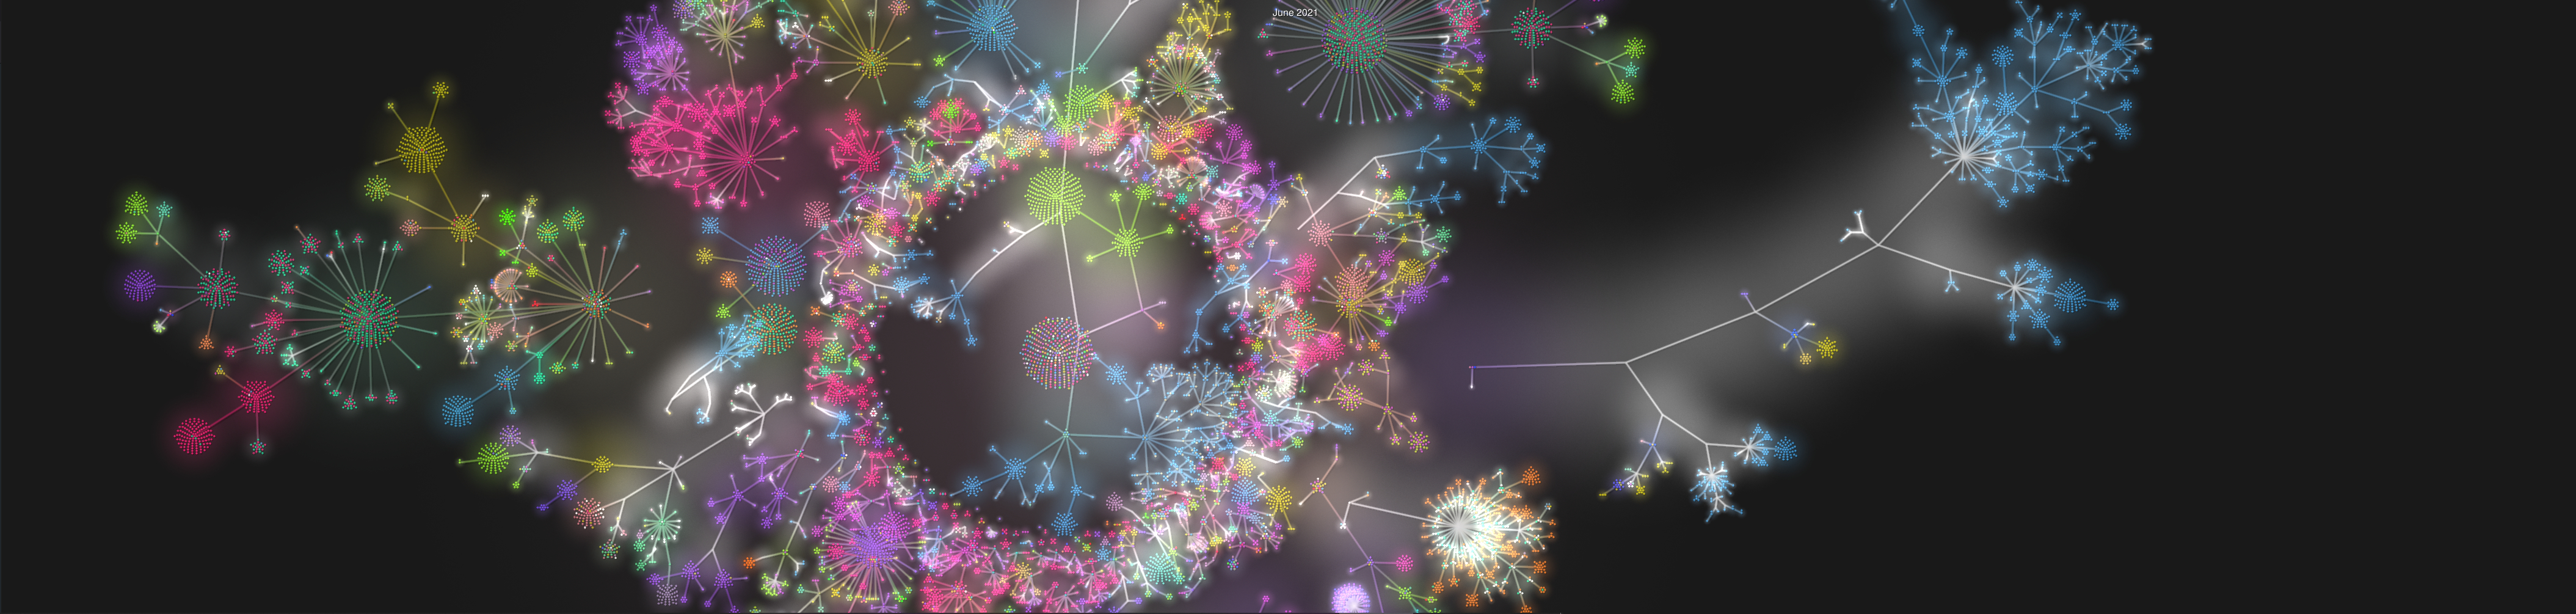
\includegraphics[width=\linewidth]{gource}
	\caption{\href{https://github.com/bitpaint/bitcoin-gources}{Bitpaint}: Contributions to the Bitcoin ecosystem. Reused with permission.}
	\label{fig:gource}
\end{figure*}
\href{https://github.com/bitcoin/}{Bitcoin core} is the main historical effort (with around a dozen major contributors guiding the direction), but there are alternatives (\href{https://github.com/libbitcoin/libbitcoin-node/wiki}{LibBitcoin in C++}, \href{https://github.com/btcsuite/btcd}{BTCD in Go}, and \href{https://bitcoinj.github.io/getting-started}{BitcoinJ in Java}), and as innovation on layer one slows, attention is shifting to codebases which interact with the base layer asset. Much more on these later.
\subsection{Mining and Energy concerns}
\subsubsection{Mining process overview}
Bitcoin mining is the process of adding public transactions into the ledger, in return for two economic rewards, paid in Bitcoin. These are the mining fee, and the block reward. The transactions which are added into the next `block' of the chain are selected preferentially based on the fee they offer, which is up to the user trying to get their transaction into the chain. This can be within the next 10 minutes (next block), or a gamble out toward 'never' depending how competitive the network is at any time. Miners try to find a sufficiently low result from a cryptographic hash function \cite{rogaway2004cryptographic}(a random process), and upon finding it, they can take their pre-prepared `block' of transactions sourced from their local queue (mempool), and add it into the chain, for confirmation by other miners. In return they take all the fees within that mined block, and whatever the block reward is at the time. When the network started the block reward was 50 Bitcoin, but has \href{https://ma.ttias.be/dissecting-code-bitcoin-halving/}{halved} repeatedly every 210,000 blocks (four years) and now stands at 6.25 BTC. The rate of mining is kept roughly at one block every 10 minutes, by a difficulty adjustment every 2016 blocks (2 weeks). This in a complex interdependent mechanism and is explained very well in \href{https://bitcoinmagazine.com/technical/how-mining-protects-the-bitcoin-network}{this article}. These components are explained in slightly more detail later.\par
\subsubsection{Energy \& policy response}
Bitcoin uses a staggering amount of energy to secure the blockchain (Figure \ref{fig:top500}), and this \href{https://www.edmundconway.com/bitcoin-money-and-the-planet/}{has climate repercussions}. A simple back of the envelope use of the \href{https://www.iea.org/reports/key-world-energy-statistics-2021/supply}{IEA total energy supply}, and the \href{https://ccaf.io/cbeci/index}{Cambridge Bitcoin energy use} estimate puts the network at \href{https://www.wolframalpha.com/input?i=153+terawatt+hours+as+percentage+of+\%28600+exa+joules+as+terrawatt+hours\%29+}{around 0.1\%} of global energy use.\par
\begin{figure*}[ht]\centering % Using \begin{figure*} makes the figure take up the entire width of the page
	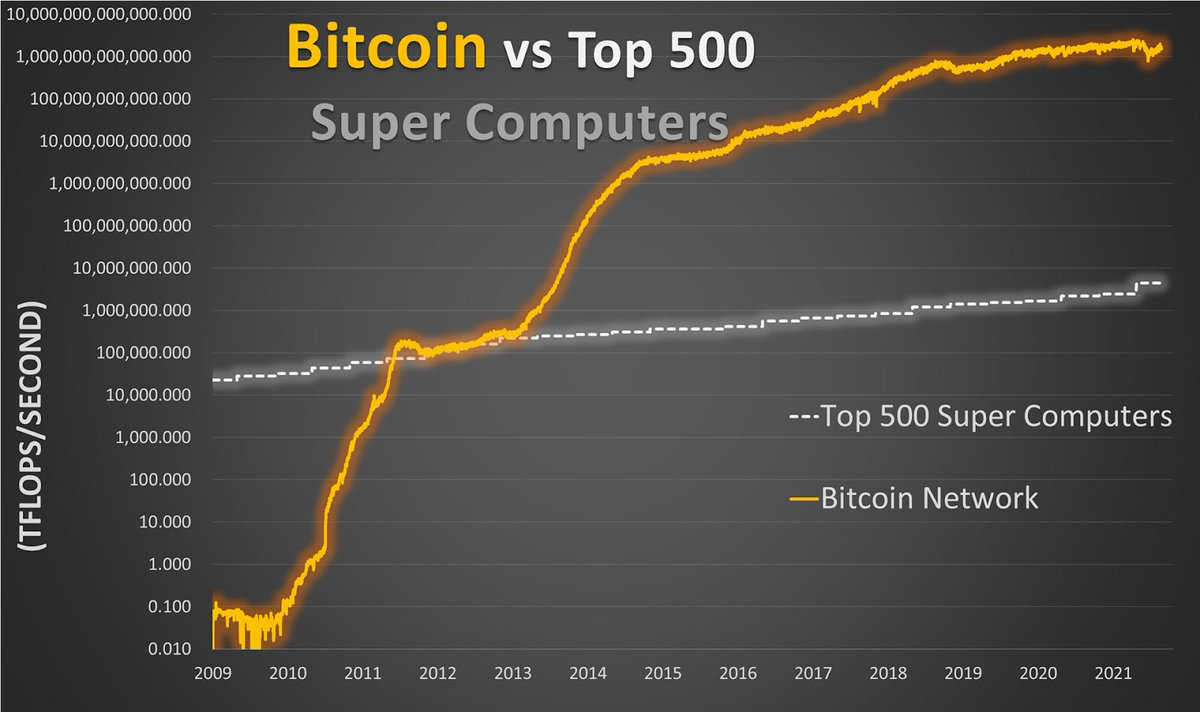
\includegraphics[width=\linewidth]{top500}
	\caption{\href{https://twitter.com/blockbain/status/1432824720727105539}{Bitcoin network vs TOP500 supercomputers}}
	\label{fig:top500}
\end{figure*}
\begin{figure*}[ht]\centering
	\includegraphics[width=\linewidth]{energycompare}
	\caption{}
	\label{fig:energycompare1}
\end{figure*}
\begin{figure*}[ht]\centering
	\includegraphics[width=\linewidth]{energycomparison}
	\caption{\href{https://bitcoinmagazine.com/business/introducing-cbei-a-new-way-to-measure-bitcoin-network-electrical-consumption}{Bitcoin Magazine}}
	\label{fig:energycompare2}
\end{figure*}
It is an \href{https://www.ruetir.com/2022/03/18/riot-whinstone-the-bitcoin-farm-with-100000-computers-that-uses-excess-energy-from-an-oil-platform-to-mine-cryptocurrencies-ruetir/}{industrial scale} global business with `mining companies' investing \href{https://ir.marathondh.com/news-events/press-releases/detail/1272/marathon-digital-holdings-bitcoin-mining-fleet-to-reach}{hundreds of millions of pounds} at a time in specialist \href{https://en.wikipedia.org/wiki/Application-specific_integrated_circuit}{ASIC} mining hardware and facilities. The latest purpose designed Intel chip \href{https://www.intel.com/content/www/us/en/newsroom/opinion/thoughts-blockchain-custom-compute-group.html#gs.pd9ofu}{touts} both Web3 and metaverse applications. This is ``proof of work'',  and is essential to the technology, and is still thought by some to be the \href{https://www.truthcoin.info/blog/pow-cheapest/}{best available option}. The \href{https://ccaf.io/cbeci/index}{Cambridge Bitcoin Energy Consumption Index} monitors this energy usage. Their \href{https://www.jbs.cam.ac.uk/insight/2022/bitcoin-mining-new-data-reveal-a-surprising-resurgence/}{2022 report} sees American mining leading globally. Even they have had a \href{https://compassmining.io/education/the-worst-of-bitcoin-mining-in-2022/}{terrible time recently} with many companies either failing or looking likely to.\par
At the end of 2022 it is thought to be the case that the only profitable miners are the large scale companies who are also providing load balancing services to energy companies. This is unusual in the history of mining, and the situation will likely change over time.
%Such businesses can mine a Bitcoin for \href{https://www.911metallurgist.com/blog/the-cost-to-mine-different-cryptocurrencies-in-every-country}{around \$5k-\$10k} per coin, so the profit margins \href{https://www.nicehash.com/profitability-calculator}{are considerable} (based on 30-40 Joule/terahash and power rate less than 5 cents/kilowatt hour and \href{https://www.tradingview.com/script/WqgcFq9o-Blockchain-Fundamentals-Electricity-Cost-of-BTC-CR/?}{excluding hardware} costs). 
This is not to say that all mining is, or should be, so concentrated. Anyone running the hashing algorithm can \href{https://twitter.com/ckpooldev/status/1485585814419812356}{get lucky} and claim the block reward. PoW ties the value of the `money' component of Bitcoin directly to energy production. This is not a new idea. Henry Ford proposed an intimate tie between energy and money to create a separation of powers from government, as can be seen in Figure \ref{fig:energyNYT}.\
\begin{figure}
  \centering
    \includegraphics[width=\linewidth]{energyNYT}
  \caption{\href{https://www.nytimes.com/1921/12/06/archives/mr-fords-energy-dollar.html}{Intimate tie between energy and money, Henry Ford}}
  \label{fig:energyNYT}
\end{figure}
The potential ecological footprint of the network has always been a concern; Hal Finney himself was \href{https://twitter.com/halfin/status/1153096538}{thinking about this issue} with a mature Bitcoin network as early as 2009, and \href{https://satoshi.nakamotoinstitute.org/posts/bitcointalk/threads/167/#35}{a debate} on the Bitcoin mailing lists called the mining process ``thermodynamically perverse''. The most cited negative analysis on the matter by Mora et al sees Bitcoin mining alone warming the planet above 2 degrees \cite{mora2018bitcoin}. \par
\href{https://electricmoney.org/}{Proponents of the technology} say that the balance shifted dramatically in 2021 with China outright banning the technology; this has forced the bulk of the energy use \href{https://docs.google.com/spreadsheets/d/1E7489rM7Q62oXwk1f4NUlMvok9noAbpYfTynY2VTyww/edit#gid=0}{toward the USA}, and away from `dirty coal' as seen in Figure \ref{fig:miningshare}. 
\begin{figure}
  \centering
    \includegraphics[width=\linewidth]{miningshare}
  \caption{Hash rate \href{https://ccaf.io/cbeci/ining_map}{suddenly migrates} from China [Reuse rights requested]}
  \label{fig:miningshare}
\end{figure}
Some adherents \href{https://docs.google.com/document/d/1N2N-5jY00cmteoY_puWI9oosM1foa4EQqsO1FFfIFR4/edit}{have proposed mitigations} \cite{cross2021greening}. As a worked example of \href{https://docs.google.com/spreadsheets/d/15e_a-D3x4fv3tglEzFmQ6TLQx0fZe6-iKO9Fc9SyISQ/edit#gid=0}{Cross and Bailey's proposal} a retail investor owning 1 BTC would have to buy around 700 shares of `CleanSpark' mining company (CLSK) to make their \href{https://docs.google.com/spreadsheets/d/1r32T8p_PHTP8S781u7PhPSwehLx2VcJTaJJKesMswD0/edit#gid=0}{holding completely neutral}.  Some more strident voices suggest that \href{https://medium.com/@magusperivallon/a-financial-hail-mary-for-the-climate-an-argument-for-bitcoin-adoption-9c58e707d0}{`ending financialisation' through use of Bitcoin} may be net positive for the environment at a macro level \cite{bitcoinisvenice}. Indeed it may \href{https://www.newsweek.com/bitcoin-mining-americas-most-misunderstood-industry-opinion-1669892}{provide a route} to support \href{https://mobile.twitter.com/DSBatten/status/1514072998881665027}{electrifying everything} through deployment of \href{https://lancium.com/solutions/}{flexible demand load}. This enables a kind of \href{https://medium.com/@theendoftheworldpartyparty/deep-bitcarbonization-c8f483716ff7}{`financial battery'} that can soak up excess capacity from overbuilt renewables (something which needs to be done). Money saving uses like \href{https://www.theguardian.com/technology/2022/feb/09/can-bitcoin-be-sustainable-inside-the-norwegian-mine-that-also-dries-wood}{drying wood}, and even heating greenhouses (\href{https://www.euronews.com/next/2022/12/14/a-bitcoin-miner-and-tulip-grower-team-up-to-reduce-costs}{ironically tulips}) show the use case of the technology as a universal subsidy in heating applications.\par
Some projects are using the financial incentive of Bitcoin to enable trials of new infrastructure. For instance; Bhutan in the Himalayas has been quietly (or secretly!) mining Bitocin for years and plans a \href{https://www.straitstimes.com/business/bhutan-plans-a-500-million-fund-for-crypto-mining-in-the-himalayas}{\$500M fund} to expand specifically Bitcoin mining. Makai Ocean engineering have partnered with Oceanbit Hawaii to trail \href{https://en.wikipedia.org/wiki/Ocean_thermal_energy_conversion}{`ocean thermal energy conversion'} as a possible power source for the Islands. Local subsidy initiatives may begin to \href{https://fortune.com/2022/08/14/bitcoin-has-plunged-but-texas-miners-are-flush-with-profits-thanks-to-an-unusual-arrangement-the-state-is-paying-them-not-to-mine/}{drive this kind of adoption} as seems to be \href{https://braiins.com/blog/bitcoin-mining-the-grid-generators}{happening in Texas}\cite{griffith2021electrify, ercotimpact2021, Menati2022} and \href{https://www.governor.nh.gov/sites/g/files/ehbemt336/files/inline-documents/sonh/cryptocurrencie-report.pdf}{New Hampshire}. Brad Jones, \href{https://www.youtube.com/watch?v=gKnRfDeFgr0}{interim CEO of the Texas grid said}:\par
\textit{``As we get more renewable generation, in particular wind [which] is operating at night ...  we have to find a home for it, otherwise we have to turn the wind down. It’s such a great resource we shouldn’t turn it down. Bitcoin mining or what some call crypto has found a way to come into our markets and take some of that wind in off-peak periods. Then when we get to peak period times they are very quick to remove themselves from the market as prices increases The fact that we can turn down whenever we need the power for other customers is fantastic. We can use that crypto currency to soak up that excess generation when there’s a lot of that, and find a home for more solar and more wind to come to our grid. Then they reduce consumption when we need that power for other customers. So it’s a great balancing act. Most other datacenters [such as] Microsoft or Amazon have other customers to serve every other day, so they can’t just turn off. But these crypto customers can. If the cost of energy gets too high they can remove themselves from the market. They are also helpful if we lose a generator. They can quickly respond to that frequency disruption and allow us to balance our grid.''}\\
Flexible load balancing is entering the \href{https://www.forbes.com/sites/jemmagreen/2023/01/27/why-no-one-saw-the-success-of-demand-response-coming/?}{mainstream news cycle} as and is gaining traction in legislative bodies. This \href{https://www.citadel21.com/bitcoin-is-the-first-global-market-for-electricity-and-will-unleash-renewables}{``global energy market revolution''} is explained by Tabatabai of Modo Energy. Incredibly Bitcoin mining in Texas is now making the grid both more reliable and cheaper for consumers.\par 
There is growing interest and adoption of so called \href{https://www.bloomberg.com/news/articles/2022-06-01/oman-backs-u-s-firm-mining-crypto-to-cut-natural-gas-flaring}{``stranded energy mining''}  which cannot be effectively transmitted to consumers, and is thereby sold at a huge discount while also \href{https://www.renewableenergyworld.com/wind-power/900mw-wind-farm-to-power-bitcoin-mining-operation/}{developing power capacity}, without the \href{https://batcoinz.com/the-renewable-energy-cannot-happen-without-bitcoin-mining\%ef\%bf\%bc/}{usual constraints} \cite{bastian2021hedging}. One such example is \href{https://gridlesscompute.com/news/}{``Gridless'' in Kenya}, which seeks to harness abundant green energy resources in rural areas with the hope of kick-starting economic growth. This feature of the network first came to popular attention in 2020 when Stevens, CEO of Stoneridge capital included the following text in a letter to shareholders within their \href{https://www.stoneridgefunds.com/documents/AnnualReport.pdf?v=4}{annual report}: \textit{``Bitcoin mining is the only profitable use of energy in human history that does not need to be located near human settlement to operate. The long-term implications of this are world changing and hiding in plain sight.''}\par
In addition to new build it is possible to \href{https://www.curbed.com/2021/07/crypto-currency-mining-old-power-plants.html}{re-purpose historic} infrastructure, and/or \href{https://www.bloomberg.com/news/articles/2022-03-24/exxon-considers-taking-gas-to-bitcoin-pilot-to-four-countries}{reducing the carbon} (or \href{https://batcoinz.com/quantifying-the-potential-impact-of-bitcoin-mining-on-global-methane-emissions-4/}{more interestingly} the methane) of existing and \href{https://www.axios.com/2023/01/27/crypto-mining-advocate-green-abandoned-gas-wells}{abandoned infrastructure}. Both the \href{https://www.weforum.org/videos/this-start-up-catches-waste-methane-to-power-data-centres}{World Economic Forum}, and UK's Department for Energy \href{https://www.contractsfinder.service.gov.uk/Notice/a99aa482-c7d1-4ec4-82fe-5c4b16827a6d}{have expressed interest} in this use case. Adam Wright of \href{https://vespene.energy/}{Vespene Energy} says: \textit{``You could either mine Bitcoin on one small landfill for a year, or you could plant 5 million trees and let them grow for 10 years - both of those are going to have the same environmental impact.''}\par
\begin{figure}
  \centering
    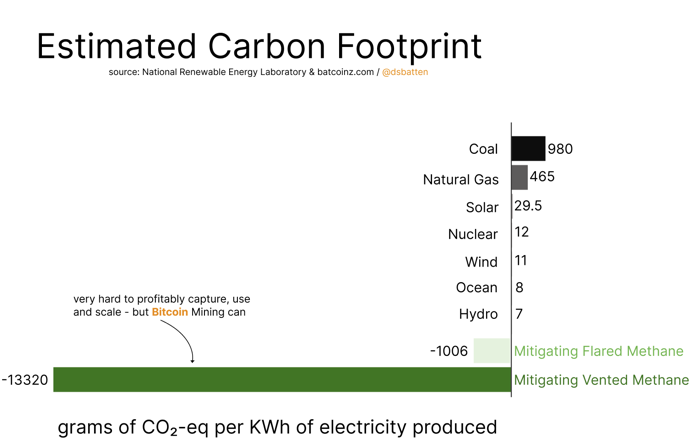
\includegraphics[width=\linewidth]{methane}
  \caption{\href{https://twitter.com/DSBatten/status/1566735902617276416}{Climate tech investor Daniel Batten asserts that methane capture could highly impactful}}
  \label{fig:methane}
\end{figure}
Cheikosman, a policy analyst for the World Economic Forum (somewhat surprisingly) \href{https://www.weforum.org/agenda/2022/03/crypto-energy-consumption/?}{wrote} \textit{``Crypto is becoming an essential part of developing a carbon-neutral energy grid and has made it economically viable to invest in, develop and build renewable energy power generation.''} 
This is explored in detail by Ibanez et al \cite{ibanez2023sok}.\par
The most cited example of building capacity before grid connection is El Salvador's `volcano mining' proposal, which is supporting their national power infrastructure plans. Uzbekistan seems to be promoting a \href{https://www.reuters.com/business/finance/uzbekistan-legalises-solar-powered-crypto-mining-2022-05-04/}{similar model} with zero tax provided the Bitcoin mining companies build out their own solar infrastructure. A more poignant example is the \href{https://www.timesunion.com/news/article/Mechanicville-hydro-plant-gets-new-life-16299115.php}{Mechanicville hydro plant in the USA}. The refurbishment of this 123 year old power plant is being funded by Bitcoin mining. This is the \href{https://www.lynalden.com/bitcoin-energy/}{``buyer of last resort''} model first \href{https://squareup.com/us/en/press/bcei-white-paper}{advanced by Square Inc}.\par
Conversely it might be that vertical integration of Bitcoin mining \href{https://bitcoinmagazine.com/business/oil-companies-partner-with-bitcoin-miners}{within legacy fossil fuel stations} gives them a new lease of life. New York State has dealt with this kind of threat by imposing a moratorium on new, fossil fuel powered mining activity. On a global stage something as portable and industrial as Bitcoin mining will have unintended impacts on fragile energy systems, as has happened in \href{https://ceobs.org/environmental-governance-in-frozen-conflicts/}{South Ossetia} and \href{https://restofworld.org/2022/crypto-miners-fleeing-kazakhstan/}{Kazakhstan} (note \href{https://thenewscrypto.com/kazakhstans-crypto-miners-to-acquire-electricity-from-russia/}{Russia has stepped into this} mess). Undeniably the \href{https://time.com/6193004/crypto-climate-impact-facts/}{consensus position} is that it's overall very negative, (with some caveats) and this will \textit{probably} persist. Perhaps though if it's happening anyway, then finding utility of the asset might mitigate the net harm.\par
More pragmatically, Baur and Oll found that \textit{``Bitcoin investments can be less carbon intensive than standard equity investments and thus reduce the total carbon footprint of a portfolio.''}\cite{baur2021bitcoin}. Perhaps of note for the near future is that KPMG whose investment was mentioned in the introduction also matched their position in the space with equivalent  carbon offsets. This may provide an investment and growth model for others.\par
The first US-based \href{https://www.businesswire.com/news/home/20230305005096/en/TeraWulf-Announces-Energization-and-Rapid-Deployment-of-Mining-Operations-at-the-Nautilus-Facility-in-Pennsylvania}{nuclear-powered Bitcoin mining facility} has just opened in Pennsylvania. The facility has been completed by Cumulus Data, a subsidiary of independent power producer Talon Energy. Talon Energy owns the adjacent 2.5 GW Nuclear Power Plant and has been dabbling in Bitcoin mining for some time, opening a zero carbon Bitcoin mining facility in collaboration with Terawolf in August 2021. The new facility will operate with a maximum capacity of 48 MW, drawing on excess power from the nuclear plant. By locating the mining facility on the combined 1200 acre campus, there is no intermediation by legacy electric transmission and distribution utilities, as the mining is directly connected to the power station. Cumulus Data is in the process of building two additional 48 MW facilities and has identified 18 additional Talon Energy sites with potential to host data centres directly connected to electricity generation infrastructure. In general, there is a shift in attitudes towards nuclear in the US. The enormous benefit to this model stems from the cots associated with scaling down atomic power output to match grid requirements. By co-locating in this way the reactor can work at highest efficiency all the time, and can earn money from the generation of Bitcoin when the grid is unable to accept the energy. It is increasingly possible to find excited talk about funding smaller more pragmatic nuclear power plants using the cost benefits of the Bitcoin mining model, though this remains untested.\par
The power commitment to the network is variously projected \href{https://www.nature.com/articles/s41558-018-0321-8}{to increase}, or \href{https://assets.website-files.com/614e11526f6630959fc98679/616df63a27a7ec339f5e6a80_NYDIG-BitcoinNetZero_SML.pdf}{level off over time}. The emission schedule of the code suggests that the energy usage will decrease exponentially over time, and indeed many analysts feel that it has peaked due to a combination of factors. It's one of the maddening unknowns of the technology how this will all pan out. The \href{https://www.forbes.com/sites/martinrivers/2022/04/03/is-bitcoin-really-that-bad-for-the-environment/?sh=6a3203427143}{industry now argues} that economic pressures mean that most of the `hashrate' is \href{https://bitcoinminingcouncil.com/q4-bitcoin-mining-council-survey-confirms-sustainable-power-mix-and-technological-efficiency/}{generated by renewable energy}\cite{blandin20203rd}. As a recent example of this trend Telsa (Elon Musk), Block (Twitters Jack Dorsey), and Blockstream (Adam Back) are teaming up to \href{https://www.cnbc.com/2022/04/08/tesla-block-blockstream-to-mine-bitcoin-off-solar-power-in-texas.html}{mine with solar energy} in Texas.\par 
Paez and Cross \href{https://uploads-ssl.webflow.com/627aa615676bdd1d47ec97d4/62f41b9ce54e014f9869efa7_OSTP.docx.pdf}{prepared a paper} for the White House Office of Science and Technology Policy, submitted through the Bitcoin Policy Institute, which is a growing thinktank for academics and industry leaders. Their summary points echo the assertions made here, but they provide rich additional referencing for those who wish to dig deeper into this:\\
\textit{\begin{itemize}
\item Bitcoin’s value—its economic value and promotion of American values and American
national interests—must frame any discussion of its environmental impact.
\item Bitcoin’s value is inherently tied to its consensus mechanism: proof of work.
\item While bitcoin mining is energy-intensive, its energy use is often overestimated and improperly characterized as a function of transaction volume.
\item Due to bitcoin’s exponentially decreasing schedule of issuance, mining’s actual emissions are likely to peak at under 1\% of global emissions, even if prices rise more than tenfold within the
decade.
\item Mining’s profile as a consumer of energy is unique: extremely cost-sensitive, and invariant
across times and locations.
\item Bitcoin mining, as a buyer of first and last resort, incentivizes the buildout of renewable power production. As a controllable load resource (CLR) bitcoin mining also strengthens the grid, allowing it to reliably function at a high level of renewable penetration.
\item Mining’s energy use is increasingly non-rival, trending towards a diet of renewables andstranded, wasted energy resources such as flared methane.
\end{itemize}}
\par%A \href{https://twitter.com/thelaserlife/status/1511354396705452035}{pseudonymous twitter user} puts this well:\par 
%\textit{``Eventually it'll seem obvious – having a mechanism to instantly monetize energy at its source was the missing ingredient to massively scale up green energy production.''}. Critics highlight the potential \href{https://www.fitchratings.com/research/us-public-finance/crypto-mining-poses-challenges-to-public-power-utilities-24-01-2022}{impact of mining on local energy} prices\cite{benetton2021cryptomining}.\par
\href{https://www.youtube.com/watch?v=6LP8G-oZnEs}{The debate} whether this consumption is `worth' it is \href{https://www.utilitydive.com/news/bitcoin-mining-as-a-grid-resource-its-complicated/617896/}{complex} and \href{https://www.aei.org/technology-and-innovation/no-hearing-on-bitcoins-energy-use-is-complete-without-nic-carter/}{rapidly evolving}. Useful examples of this are:
\begin{itemize}
\item the \href{https://www.zerohedge.com/crypto/questionable-ethics-anti-bitcoin-esg-junk-science}{online pushback} to an academic article by PhD candidate de Vries et al. \cite{de2022revisiting}
\item the assertion that the widely cited Mora er al. paper in Nature \cite{mora2018bitcoin} was based on an \href{https://twitter.com/NateHawaii/status/1460706785216450560}{undergraduate class discussion}, and has had an outsized effect on global policy. 
\item a \href{https://rebrand.ly/v8qq1sx}{paper from the Bitcoin Policy Institute}, 
\item and the industry \href{https://bitcoinminingcouncil.com/wp-content/uploads/2022/05/Bitcoin_Letter_to_the_Environmental_Protection_Agency.pdf}{open letter to the EPA}.\par
\item this well considered \href{https://twitter.com/jyn_urso/status/1508899761319038983}{Twitter thread} by climate scientist Margot Paez.
\end{itemize}
It is somewhat confusing that positive views are coming only from diverse and non-specialist voices in the community, and never the academic community, but the shortcomings they point out in the supposedly considered articles such as Mora et al \cite{mora2018bitcoin} are easily verified. Academia seems \href{https://bitcoinmagazine.com/culture/bitcoin-could-never-be-invented-in-a-university}{poorly positioned} to pivot to this subject, as an ethical bar has to be established before research can commence, and the field is too new to make this an affordable task. This stuff is existentially important to the whole technology. Is a trillion dollar asset which \href{https://www.theheldreport.com/p/bitcoin-vs-gold}{potentially replaces} the money utility of gold, but doesn't need to be stored under guard in vaults (Figure \ref{fig:goldmanVgold}), worth the equivalent power consumption of clothes dryers in North America? Probably not with the current level of adoption, but this is an experiment in replacing global money. If that were to happen then Bitcoin would be around 50 times more efficient than the current system according to Khazzaka \cite{khazzaka2022bitcoin}. To be clear it's not the position of this book that replacing Fiat money is a good idea, but the experiment is being run regardless. This is explored in it's own chapter later.\par
It seems possible that six value propositions are therefore emerging:
\begin{itemize}
\item Bitcoin the speculative asset (or greater fool bubble \cite{de1990positive}). Nations such as the USA, who own 30\% of the asset have bid up the price of the tokens during a period of very cheap money, and this has led to a high valuation for the tokens, with a commensurately high network security through the hash rate (mining). This could be a speculative bubble, with the asset shifting to one of the other valuations below. There is more on this subject in the money section later.
\item Bitcoin the monetary network, and `emerging market' value transfer mechanism. This will be most useful for Africa (especially Nigeria), India, and South America. There is no sense of the ``value'' of this network at this time, but it's the aspect we need for our collaborative mixed reality application. For this use the price must simply be high enough to ensure that mining viably secures the network. This security floor is unfortunately a `known unknown'. If a global Bitcoin monetary axis evolves (as in the Money chapter later) the network would certainly require a higher rate than currently, suggestive of a higher price of token to ensure mining \cite{Wouters2022}.
\item Bitcoin's value in terms of `sunk opportunity cost'. This refers to the value that could have been generated if the resources invested in a particular activity had been utilised elsewhere. In the context of Bitcoin, this includes the investments made in mining equipment, power, facilities, and the hiring of skilled personnel to maintain the operations. The sunk opportunity cost of Bitcoin can be substantial. It can be argued that the value of Bitcoin must take this cost into consideration, as the resources could have been allocated to other productive sectors or investments \cite{chiu2017economics}. Of course, there remains the infamous sunk cost fallacy, which refers to the tendency of individuals or organizations to continue investing in a project or decision based on the amount of resources already spent, rather than evaluating the current and future value of the investment. This indeed tends to lead to a cyclical boom and bust dynamic in the industrial mining communities. The ultimate fallacy would occur if miners or investors continued to invest in mining equipment and operations solely because of the resources that have already been spent on them, and the asset simply crashes to nothing from here. It's a shaky justification because it assumes the future is the same as the past.
\item Bitcoin as a flexible load in power distribution systems, and methane mitigation `asset', and `subsidised heater' for varied applications such as growing and drying. Again there is no price against this, but we can perhaps grossly estimate it at around half the current hash rate if 50\% of the network is currently green energy. This would imply a price for the asset roughly where it is now (ie, not orders of magnitude higher or lower). 
\item The 2023 global bank runs have awoken some companies to the risks of access to cash flows in a potential crisis \cite{jiang2023monetary}. Access to a small cache (in corporate treasury terms) of a highly liquid \& tradable asset could allow continuity of payroll in a `24/7' global context. This could avoid or at least mitigate the panic which ensues in companies when banks are forces to suddenly wind up their operations.  
\item Amusingly \href{https://www.epsilontheory.com/in-praise-of-bitcoin/}{Ben Hunt suggests} in an online article that the true value of Bitcoin can be couched in terms of it's value simply as `art'. The posits that at this time the narrative is simply so seductive and powerful that people (being people) are choosing to value their involvement in the economics of the space as they might a work of art. It's a fascinating idea, and intuitively, probably it's right. 
\end{itemize}
\begin{figure}
  \centering
    \includegraphics[width=\linewidth]{goldmanvgold}
  \caption{Goldman suggest growth opportunity and potential demonetisation of gold?}
  \label{fig:goldmanVgold}
\end{figure}
Legislators globally, are \href{https://www.lopp.net/bitcoin-information/legal.html}{starting to codify} their positions on proof of work as a technology (including Bitcoin). US States are variously \href{https://capitol.texas.gov/tlodocs/88R/billtext/html/HC00089I.htm}{supporting} or constricting the technology, according to \href{https://www.ncsl.org/research/financial-services-and-commerce/cryptocurrency-2021-legislation.aspx}{state legislatures}. Notably New York has \href{https://www.nysenate.gov/legislation/bills/2021/A7389}{banned new carbon intensive} mining facilities for 2 years, while rust and farm belt states with energy build-out problems are \href{https://financialpost.com/fp-finance/cryptocurrency/texas-governor-abbott-turns-to-bitcoin-miners-to-bolster-the-grid-and-his-re-election}{providing incentives} and passing legislation to protect \href{https://www.arkleg.state.ar.us/Bills/Detail?id=hb1799}{mining datacenters}. At the federal level the white house has strongly signalled their concerns about the sector \href{https://www.whitehouse.gov/wp-content/uploads/2023/03/ERP-2023.pdf}{in a report}. Many of the points in the report are fair, and true, and reflect things said in this book (which pre-dates the report). It's worth picking out the conclusion of that section verbatim: \textit{``Innovation in financial services brings both risks and opportunities for the broader economy. It can challenge business models and existing industries, but it cannot challenge basic economic principles, such as what makes an asset effective as money and the incentives that give rise to run risk. Although the underlying technologies are a clever solution for the problem of how to execute transactions without a trusted authority, crypto assets currently do not offer widespread economic benefits. They are largely speculative investment vehicles and are not an effective alternative to fiat currency. Also, they are too risky at present to function as payment instruments or to expand financial inclusion. Even so, it is possible that their underlying technology may still find productive uses in the future as companies and governments continue to experiment with DLT. In the meantime, some crypto assets appear to be here to stay, and they continue to cause risks for financial markets, investors, and consumers. Much of the activity in the crypto asset space is covered by existing regulations and regulators are expanding their capabilities to bring a large number of new entities under compliance (SEC 2022). Other parts of the crypto asset space require coordination by various agencies and deliberations about how to address the risks they pose (U.S. Department of the Treasury 2022a). Certain innovations, such as FedNow and a potential U.S. CBDC, could help bring the U.S. financial infrastructure into the digital era in a clear and simple way, without the risks or irrational exuberance brought by crypto assets. Hence, continued investments in the Nation’s financial infrastructure have the potential to offer significant benefits to consumers and businesses, but regulators must apply the lessons that civilization has learned, and thus rely on economic principles, in regulating crypto assets.''}\par
Reading between the lines suggest that strong regulation is coming. Indeed the \href{https://www.sec.gov/Archives/edgar/data/1679788/000167978823000051/coin-20230322.htm}{SEC is now suing} the major tech company in the space, Coinbase, while closing a bank servicing the sector, and signalling that stablecoins may be unregistered securities in law. The report itself has no `teeth' but is likely a sign of things to come. There is purportedly \$2.4B \href{https://docs.house.gov/meetings/AP/AP23/20230329/115576/HHRG-118-AP23-TTF-GenslerG-20230329.pdf}{entering the regulation ecosystems} to enhance regulatory oversight. In actual fact, because of the nature of the federation of states it is likely that a variety of different approaches in law will be taken across the geography and the sector seems to have responded with a shrug. As an aside the report contains an excellent taxonomy of digital assets from Hoffman (Figure \ref{fig:PresidentTaxonomy}).\par
\begin{figure}
  \centering
    \includegraphics[width=\linewidth]{presidenttaxonomy}
  \label{fig:PresidentTaxonomy}
\caption{Taxonomy of digital assets Hoffman 2022}
\end{figure}
Conversely the recent ``\href{https://www.whitehouse.gov/ostp/news-updates/2022/09/08/fact-sheet-climate-and-energy-implications-of-crypto-assets-in-the-united-states/}{Climate and energy implications}'' report is parts positive and parts negative about proof of work, and leaves the door open to a legislative clampdown. This is most notable in a \href{https://www.whitehouse.gov/cea/written-materials/2023/05/02/cost-of-cryptomining-dame-tax/}{White House proposal} to tax Bitcoin mining at 30\%, a plan which will destroy much of the US based mining industry over the coming years. Carter provides a \href{https://medium.com/@nic__carter/comments-on-the-white-house-report-on-the-climate-implications-of-crypto-mining-8d65d30ec942}{detailed response} to the tardy scientific analysis in the report. Perhaps most interestingly it notes the potential of methane mitigation as mentioned earlier. It is conceivable that methane mitigation alone could provide a route forward for the technology. The report says:
\textit{``The crypto-asset industry can potentially use stranded methane gas, which is the principal component of natural gas, to generate electricity for mining. Methane gas is produced during natural gas drilling and transmission, and by oil wells, landfills, sewage treatment, and agricultural processes. Methane is a potent GHG that can result in 27 to 30 times the global warming potential of CO2 over a 100-year time frame, and is about 80 times as powerful as CO2 over a 20-year timeframe. Reducing methane emissions can slow near-term climate warming, which is why the Biden-Harris Administration released the U.S. methane emissions reduction action plan in 2021. Venting and flaring methane at oil and natural gas wells wastes 4\% of global methane production. In 2021, venting and flaring methane emitted the equivalent of 400 million metric tons of CO2, representing about 0.7\% of global GHG emissions. This methane is vented or flared, because of the high cost of constructing permanent pipelines or electricity transmission that could transport the methane or its potential electricity generation from remote oil and gas operations to end-users, or because of the high cost of installing equipment on older landfills. Crypto-asset companies are now exploring ways to use electricity generation from vented and flared methane at oil and gas wells and at landfills.
While the EPA and the Department of the Interior have proposed new rules to reduce methane for oil and natural gas operations, crypto-asset mining operations that capture vented methane to produce electricity can yield positive results for the climate, by converting the potent methane to CO2 during combustion. Mining operations that replace existing methane flares would not likely affect CO2 emissions, since this methane would otherwise be flared and converted to CO2. Mining operations, though, could potentially be more reliable and more efficient at converting methane to CO2. While such operations can reduce wasted methane, another option is low-cost recovery of methane using existing vapor capture technologies at oil and gas wells, which can reduce global methane emissions up to 50\% by 2030.''}\par
The EU has just voted to add the whole of `crypto', including PoW, to the EU taxonomy for sustainable activities. This EU wide classification system provides investors with guidance as to the sustainability of a given technology, and can have a meaningful impact on the flows of investment. With that said the report and addition of PoW is not slated until 2025, and it is by no means clear what the analysis will be by that point. Meanwhile they're tightening controls of transactions, on which there will be more detail later. For it's part the European Central Bank has come out \href{}{in favour of strong constraints} on crypto mining. They use the \href{https://medium.com/crescofin/the-reports-of-bitcoin-environmental-damage-are-garbage-5a93d32c2d7}{widely discredited} ``digiconimist'' estimates to assert that mining operations are \href{https://www.ecb.europa.eu/pub/financial-stability/macroprudential-bulletin/html/ecb.mpbu202207_3~d9614ea8e6.en.html}{disproportionately damaging to the environment}.  \par
We have seen that China has cracked down hard on the technology, banning mining and pressuring holders of the assets. They have unwound this somewhat, and based on past experience it seems that they will continue to nuance their position as they seek adoption of their own digital currency. As much as 20\% of all mining activity is now suspected to take place within China.\par
In India there has been confusion for years as more ``local'' law vies with confusing central government signalling. It has variously been banned and unbanned, and is now subject to punitive tax. The central bank of India is \href{http://164.100.24.220/loksabhaquestions/annex/179/AS10.pdf}{strongly in favour} of a complete ban. Ajay Seth, secretary of the Finance Ministry's Department of Economic Affairs recently said \textit{``We have gone through a deep dive consulting with not just the domestic and institutional stakeholders but also organizations like IMF and World Bank.... Simultaneously we are also beginning our work for some sort of a global regulation (to determine) what role India can play... Whatever we do, even if we go to the extreme form, the countries that have chosen to prohibit, they can't succeed unless there is a global consensus''}\par
It feels like a global political response is just around the corner, but reputable voices in the community suggest that it always feels this way. There is more detail on this in Money chapter later in the book.
\subsection{Technical overview}
This section could be far more detailed, but this is pretty complex stuff. Instead, there's plenty of \href{https://github.com/bitcoinbook/bitcoinbook}{books and websites} that do a more thorough job, if the reader is interested. Each subsection will include a good external link where more depth can be found. This whistle stop tour of the main components of the protocol should provide enough grounding, but it's not essential reading for non technical readers.\par
\subsubsection{ECDSA / SHA256 / secp256k1}
These technologies tend to use the same underpinning \href{https://curves.ulfheim.net/}{elliptic curve cryptography}, and it makes sense to unpack this here just once, only in the context of Bitcoin, as this will be the main focus of our attention.\par
Public keys are a huge number used in conjunction with an algorithm to encrypt data. This allows a remote party to interact with an actor on the network whose private keys can decrypt that same data.\par
In Bitcoin the ECDSA algorithm is used on the \href{https://en.bitcoin.it/wiki/Secp256k1}{secp256k1} elliptic function to create a trapdoor. This (essentially) one way mathematical operation was originally the ``discrete log problem'' and part of the research in cryptography by Diffie and Hellman \cite{diffie1976new}. This is what binds the public and private keys in a key pair (the foundation of the whole space).\par 
In their mathematical construct a modulus operator creates an infinite number of possible variations on operations which multiply enormous exponential numbers together, in different orders, to create key pairs. In order to reverse back through the `trapdoor' a probably impossible number of guesses would have to be applied.\par
Latterly, elliptic curves such as the secp256k1 curve used in Bitcoin have substantially simplified the computation problems. Rather than exponentials used by Diffie Helmman instead a repeated operation is applied to an elliptic curve function, and this itself creates a discrete log problem trapdoor in maths, far more efficiently. Figure \ref{fig:ECDSA} suggests how this works. \par
This makes it easier, faster, and cheaper to provide secure key pairs on basic computational resources. Elliptic curve solutions are not \href{https://safecurves.cr.yp.to/}{`provably' secure} \cite{gayoso2018secure} in the same way as the Diffie-Hellman approach, and the security of this system is very sensitive to the randomness which is applied to the operation. Aficionados of Bitcoin use dice rolls or \href{https://www.hackster.io/news/alex-waltz-s-quantum-random-number-generator-for-bitcoin-uses-radioactive-decay-and-a-raspberry-pi-25a75316220f}{even more exotic} means to add entropy (randomness) when creating keys. This really isn't necessary, the software does this well enough.\par  
ECDSA has already been replaced by the more efficient Schnorr signature method \cite{schnorr1989efficient} which uses the same mathematical curve so is backward compatible. This will take some time for organic adoption, and ECDSA will never be deprecated.\par
\begin{figure}
  \centering
    \includegraphics[width=\linewidth]{ECDSA}
  \caption{Given a start point on the curve and a number of reflection operations it's trivial to find a number at the end point, but impossible to find the number of \href{https://github.com/bitcoinbook/bitcoinbook/blob/develop/ch04.asciidoc}{hops} from the two end points alone. (CC Mastering Bitcoin second edition)}
  \label{fig:ECDSA}
\end{figure}
\subsubsection{Addresses \& UTXOs}
Ethereum has addresses which transactions flow in and out of. This is synonymous to a bank account number and so makes intuitive sense to users of banks. This is not the case in Bitcoin.\par
Bitcoin is a UTXO model blockchain. UTXO stands for unspent transaction output, and these are `portions' of Bitcoin created and destroyed as value changes hands (through the action of cryptographic keys). They are the basis of the evolving ledger. This process is described well by Rajarshi Maitra in \href{https://medium.com/bitbees/what-the-heck-is-utxo-ca68f2651819}{this post}.\par
\textit{``Every Transaction input consists of a pointer and an unlocking key. The pointer points back to a previous transaction output. And the key is used to unlock the previous output it points to. Every time an output is successfully unlocked by an input, it is marked inside the blockchain database as `spent'. Thus you can think of a transaction as an abstract “action” that defines unlocking some previous outputs, and creating new outputs.\\
These new outputs can again be referred by a new transaction input. A UTXO or `Unspent Transaction Output' is simply all those outputs, which are yet to be unlocked by an input.\\
Once an output is unlocked, imagine they are removed from circulating supply and new outputs take their place. Thus the sum of the value of unlocked outputs will be always equal to the sum of values of newly created outputs (ignoring transaction fees for now) and the total circulating supply of bitcoins remains constant.''}\par
Fresh UTXOs are created as coinbase transactions, rewarded to miners who successfully mine a block. These can be spent to multiple output as normal. This is how the supply increases over time.
\subsubsection{Bitcoin script and miniscript}
A Bitcoin script is a short chunk of code written into each transaction which gives conditions for the next UTXO transfer (spend). Bitcoin script is a programming language invented by Satoshi Nakamoto as part of the Bitcoin system. It's a stack-based language, similar to reverse Polish notation, used to encode transactions and specify the conditions under which a Bitcoin address can be spent. Bitcoin script has 256 op codes, some of which are deprecated or can cause the program to fail.\par
Miniscript is a higher-level language that makes it easier to write robust Bitcoin smart contracts on chain. It smooths out the rough edges of Bitcoin script and makes it more accessible for non-technical users to understand and use. Miniscript provides a more intuitive way to specify spending conditions, making it easier for users to create smart contracts without needing to be an expert in programming languages like Rust or C++. Miniscript takes the basket of 256 op codes in Bitcoin script and simplifies them, making the most commonly used op codes more accessible and usable for average users. The \href{https://bitcoin.sipa.be/miniscript/}{limited scripting language} and the features built into wallets on top, allow for some clever additional options beside receiving and spending. In fact, some of the more innovative features such as discrete log contracts (detailed later) are quite powerful, and can interact with the outside world. Scripts allow spends to be contingent on multiple sets of authorising keys, time locks into the future, or both.\par 
Time locks can be either block height-based or wall time-based, but Miniscript ensures that the user has to choose one or the other within a single Bitcoin script. This is because some of the time lock opcodes like "check lock time verify" (CLTV) and "op sequence verify" change their behavior based on whether the code is four or five bytes long. Miniscript removes these quirks by providing a unified and more intuitive way to write smart contracts. An example of Miniscript's functionality is a decaying multi-sig where a five of five multi-sig can be changed over time to a four or five multi-sig, or a three of five multi-sig, in case one or two keys are lost. This provides the user with more control and flexibility over their money and allows for contingencies in case of loss events. Additionally, Miniscript enables users to have \href{https://bitcoindevkit.org/bdk-cli/playground/}{more control over their funds} by setting rules when money is put into a Bitcoin address, as well as allowing for corporate governance situations. Miniscript can also be used for inheritance planning, where a child's key can be made to activate after a certain number of blocks have passed, creating a "dead man switch" functionality on the chain.\par
Overall, Miniscript enables users to have more control and flexibility over their funds, making Bitcoin smart contracts more robust and secure, but it's important to note that this is new technology and not yet integrated into user wallets.
\subsubsection{Halving}
As mentioned eariler, roughly every four year the `block reward' given to miners halves. This gives the issuances schedule of Bitcoin; \href{http://bashco.github.io/Bitcoin_Monetary_Inflation/}{it's monetary inflation}. This `controlled supply' feature was added to emulate the growth of physical asset stocks through mining. It's exhaustively \href{https://en.bitcoin.it/wiki/Controlled_supply}{explained elsewhere} and is somewhat immaterial to our transactional use case in metaverse applications.
\subsubsection{Difficulty adjustment}
The difficult adjustment (also mentioned earlier) shifts the difficulty of the mining algorithm globally to re-target one new block every 10 minutes. This means that adding a glut of new mining equipment will increase the issuance of Bitcoins, in favour of the new mining entity, for up to 2 weeks, at which point the difficulty increases, the schedule resets, and the advantage to the new miner is diffused. Equally this protects the network against significant loss of global mining hashrate, as happened when China comprehensively banned mining. Again, this is explained in \href{https://en.bitcoin.it/wiki/Difficulty}{more detail} elsewhere.
\subsubsection{Bitcoin nodes }
The Bitcoin network can be considered a triumvirate of economic actors, each with different incentives. These are:
\begin{itemize}
\item Holders and users of the tokens, including exchanges and market makers, who make money speculating, \href{https://en.wikipedia.org/wiki/Arbitrage}{arbitraging}, and providing liquidity into the network. Increasingly this is also real `money' users of BTC, earning and spending in pools of circular economic activity. Perversely Bitcoin as a money is the fringe use case at this time.
\item Miners, who profit from creation of new UTXOs, and receive payments for adding transactions to the chain. In return they secure the network by validating the other miners blocks according the rules enforced by the node operators.
\item Node operators, \href{https://www.truthcoin.info/blog/measuring-decentralization/}{who enforce the consensus} rule-set, which the miners must abide by in order to propagate new transaction into the network. In return node operators optimise their trust minimisation, and help protect the network from changes which might undermine their speculation and use of the tokens \cite{blocksizewars}.
\end{itemize}
There are currently around \href{https://bitnodes.io/}{15,000 Bitcoin nodes} distributed across the world. 
Since IT engineer \href{https://stadicus.com/}{Stadicus} released his \href{https://raspibolt.org/backstory.html}{Raspibolt guide} in 2017 there has been an explosion of small scale Bitcoin and Lightning node operators. 
Around thirty thousand Raspberry Pi Lightning nodes (which are also by definition Bitcoin nodes) run one of a big selection of \href{https://github.com/bavarianledger/bitcoin-nodes}{open source distributions}. We will build toward our own throughout the book.
\begin{comment}
with the most noteworthy explained alongside their stand-out feature-set:
\begin{itemize}
\item \href{https://github.com/rootzoll/raspiblitz}{Raspiblitz} offers fully opensource lightning focused functionality with a touchscreen display
\item \href{https://github.com/mynodebtc/mynode}{Mynode} focuses on ease of use through a web interface and has many modules which users can try out.
\item \href{https://github.com/getumbrel/umbrel-os}{Umbrel} is a more user friendly multi purpose node allowing access to a suite of Bitcoin and self sovereign individual tools.
\item \href{https://wiki.ronindojo.io/}{RoninDojo} is designed for use alongside the privacy focused \href{https://samouraiwallet.com/}{Samourai mobile wallet}.
\item \href{https://github.com/fort-nix/nix-bitcoin}{nix-bitcoin} focuses on security of the underlying operating system by building on NixOS.
\item \href{https://nodl.it}{NODL} is a premium prebuilt node focusing on security of the more performant hardware, and underlying operating system. It offers additional privacy tools.
\item \href{https://store.start9labs.com/collections/embassy}{Start9 Embassy} is a small form factor prebuilt unit at a lower price. It is a venture capital funded project with a more restrictive license but offers a suite of easy to use self sovereignty tools including Bitcoin. 
\item \href{https://www.osinteditor.com/NXN/mp_march28_f3/index.html}{The CLBoss plugin} can be combined with `Core Lightning' to automate much of the management, and is a contender for our deployment too.
\end{itemize}
This is as good a time as any to start shaping a mission statement: \textbf{This book builds toward a new collaborative mixed reality suite of tools, that utilises the nix-bitcoin distribution for the Bitcoin node}. There's a lot of components that haven't been covered yet, but nix-bitcoin is the first selected piece of open source software.
%\href{https://nydig.com/research/nydig-bitcoin-101}{Consider  mining the NYDIG primer for information}
\end{comment}
\subsubsection{Wallets, seeds, keys and BIP39}
In all the cryptographic systems described in this book everything is derived from a private key. This is an enormous number, and the input to the trapdoor function described earlier. As usual, it's beyond the scope of this book to `rehash' the detail. Prof Bill Buchanan OBE has a \href{https://medium.com/asecuritysite-when-bob-met-alice/can-i-derive-the-private-key-from-the-public-key-ba3609256ec}{great post} on the basic version of this process.\par
In modern wallets, private keys (and so too their public keys), and addresses, are generated hierarchically. This is all part of \href{https://github.com/bitcoin/bips/blob/master/bip-0032.mediawiki}{BIP-0032}. It starts with a single \href{https://www.wolframalpha.com/input?i=2\%5E512}{monstrously large} number of up to 512 bits. From this are crafted Hierarchical Deterministic (HD) wallets, which use `derivation paths' to make a tree of public/private key pairs, all seeded from this first number. This means that knowing the initial number, and the derivation path applied to it (just another number), wallets can search down the tree of derivations and find all the possible addresses. In this way a whole group of active addresses belonging to an entity can be held conveniently in one huge number (a concatenation of the input and path). This is the seed. Seeds are even more conveniently abstracted into a mnemonic called a seed phrase. Anyone interacting with these systems will see a 12 word (128 bits of entropy which is considered to be \href{https://twitter.com/adam3us/status/1433375602808066049}{`enough'}) or 24 word (256 bit) seed phrase. That phrase accesses the whole of the assets stored by that entity in the blockchain under it. A master key. These seeds can be \href{https://vault12.com/securemycrypto/cryptocurrency-security-how-to/dice-crypto-recovery-seed/}{generated by hand} with dice, remember it's just a huge number and the onward cryptography at play here.\par
An address in Bitcoin is derived from the public/private key pair. Again this is a one way hash function. The public/private keys can't be found from the address. Addresses are really only a thing in wallets. They contain the element necessary to interact with the UTXOs. Many UTXOs can reside under an address, in that they just share the same keys. Wallets and nodes can monitor the blockchain to see transactions that `belong' to addresses owned by the wallet, then they can perform unlocking of those funds to move them, through operations on the UTXOs via keys.\par
\subsubsection{Custody}
The topic of `custody' of Bitcoin (addresses,UTXOs) can be confusing at first. This is another area where there's a lot of detail available, but not all of it is appropriate because increased complexity increases risk. Broadly though it's important to remember that ownership of a UTXO is passed around using signing keys, which are functions of wallets. Wallets themselves don't contain Bitcoin, they contain keys. The simplest approach is a software wallet. This is an application on a device, which stores the private keys, and manages signing of transactions which go onto the blockchain. It's beyond the scope of this book to review or suggest software in detail, but \href{https://bluewallet.io/}{Bluewallet} on mobile devices, and \href{https://sparrowwallet.com/}{Sparrow Wallet} on desktop devices provide rich basic functionality if a reader wishes to get started immediately. Note that these software wallets send your extended public key (the path of those keys) to the wallet providers server, for the monitoring of the blockchain to happen on it's behalf. They're updated by the software vendor, not the blockchain direct. To get this to `privacy best practice' commensurate with the aim of this book it's necessary to run a full node as detailed above, and connect the wallet software to that on a secure or local connection.\par
So called \href{https://unchained.com/blog/best-bitcoin-hardware-wallets/}{hardware wallets} should perhaps be termed signing devices. A \href{https://www.reddit.com/r/Bitcoin/comments/z27jg8/comment/ixfj0w4/?}{reddit user} simplifies this concept very well: \textit{``Your hardware wallet is a safe that holds a key. Your bitcoin is in a mailbox that anyone can look at or put more bitcoin into, but nobody can take the bitcoin out unless they have the key stored in your safe. The 24 word seed phrase are the instructions needed to cut a new key.''}. Rather than store Bitcoin they store the private key in a more secure way, in a device which interacts with a computer or phone. More recently the hardware and associated software of such devices are building in \href{https://content.trezor.io/coinjoin}{much needed privacy technology}. Remember that all transactions on the Bitcoin blockchain are public. Interestingly these privacy technologies are subject to chain surveillance under the terms of their agreements, and companies like \href{https://www.wired.com/story/bitcoin-fog-roman-sterlingov-blockchain-analysis/}{Chainalysis rightly draw criticism}.\par 
We prefer hardware signing devices which can scan in the seed each time themselves as is the case with opensource \href{https://seedsigner.com/}{``seedsigner''}, which also supports Nostr delegation (Figure \ref{fig:seedsigner}). This makes the device perfect for management of all of our proposed metaverse keys.\par

\begin{figure}
  \centering
    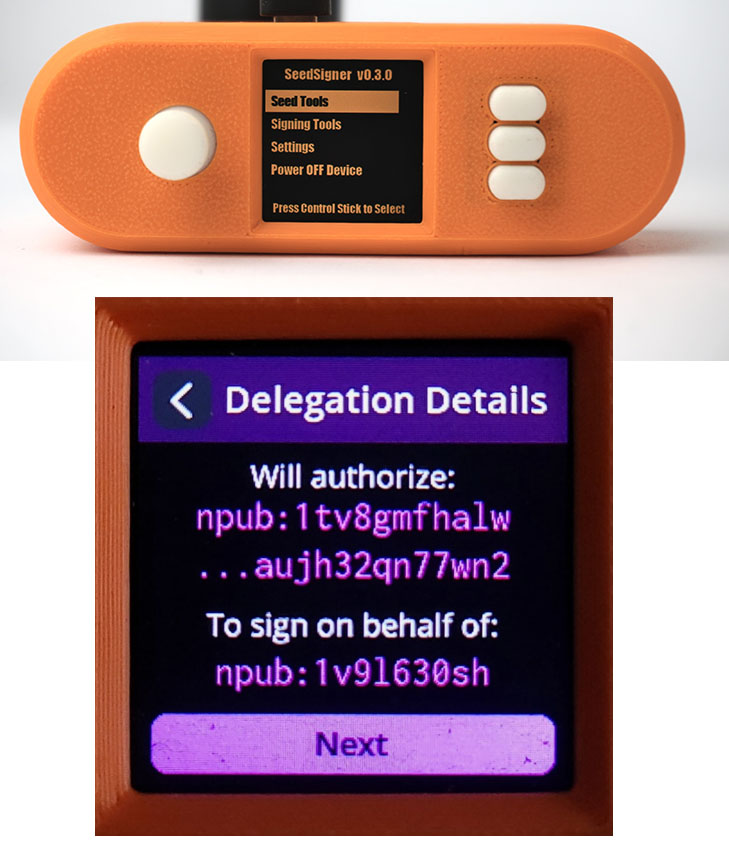
\includegraphics[width=\linewidth]{seedsigner}
  \caption{Seedsigner is an inexpensive open source project which scans the master seed in from a QR code to enable signing. One device can run a quorum based wallet (multisig) and manage Nostr identity.}
    \label{fig:seedsigner}
\end{figure}
For higher security it's possible to combine hardware and software wallets (signing devices) to provide a quorum of signatures required to move funds. More exotic still are \href{https://fedimint.org/}{proposals like ``Fedimint''} which allows groups such as families or villages to leverage their personal trust to co-manage Bitcoin. What is not/rarely secure is leaving Bitcoin with a custodian such as an exchange as they simply issue you with an IOU and may abscond. In building toward a proposal for a product in this book it would be simple for us to build a metaverse which users simply paid to use. This is the norm up to now. Representative money would flow around in the metaverse and be changed back like game money at some point. This is not what we wish to promote, so everything will be a variation on ``self-custody'', minimising third party trust for users.
\subsection{Upgrade roadmap}
\subsubsection{Taproot}
`Taproot' is the most recent upgrade to the Bitcoin network. It was first \href{https://lists.linuxfoundation.org/pipermail/bitcoin-dev/2018-January/015614.html}{described in 2018} on bitcoin-dev mailing list, and become \href{https://github.com/bitcoin/bips/blob/master/bip-0341.mediawiki}{BIP-0341} in 2019. It brings improved scripting, smart contract capability, privacy, and Schnorr signatures \cite{schnorr1989efficient}, which are a maximally efficient signature verification method. The network will always support older address types. It is rare to get such a large update to the network, and deployment and upgrade was carefully managed over several months under BIP-0008. Uptake will be slow as wallet manufacturers and exchanges add the feature. It can be considered an \href{https://transactionfee.info/charts/transactions-spending-taproot/}{upgrade in progress (0.3\%)}. Aaron van Wirdum, a journalist and educator in the space describes Taproot in detail in \href{https://bitcoinmagazine.com/technical/taproot-coming-what-it-and-how-it-will-benefit-bitcoin}{an article}.\par
\subsubsection{AnyPrevOut}
\href{https://anyprevout.xyz}{BIP-0118}, is a ``\href{https://en.bitcoin.it/wiki/Softfork}{soft-fork} that allows a transaction to be signed without reference to any specific previous output''. It enables ``Eltoo, a protocol that fulfils Satoshi's vision for nSequence''\par
This is Lightning Network upgrade technology in the main. The Eltoo \href{https://blockstream.com/eltoo.pdf}{whitepaper} or this more \href{https://fiatjaf.alhur.es/ffdfe772.html}{readable explanation} from developer fiatjaf go into detail.\par 
\subsubsection{CheckTemplateVerify}
\href{https://utxos.org/}{BIP-0119} is ``a simple proposal to power the next wave of Bitcoin adoption and applications. The underlying technology is carefully engineered to be simple to understand, easy to use, and safe to deploy''. At it's most basic it is a constructed set of output hashes, creating a Bitcoin address, which if used, can only be spent under certain defined conditions. This is a feature called `covenants'. It enables a feature called `vaults' which provides \href{https://github.com/jamesob/simple-ctv-vault/blob/7dd6c4ca25debb2140cdefb79b302c65d1b24937/README.md}{additional safety features} for custodians. There is currently \href{https://blog.bitmex.com/op_ctv-summer-softfork-shenanigans/}{some debate about the activation process}, and the feeling is that it won't happen (soon).
\subsubsection{Blind merge mining}
BIP-0301 allows `other' chains transactions to be mined into Bitcoin blocks, and for miners to take the fees for those different chains, without any additional work or thoughts by the miners. This is also a prerequisite for Drivechains (mentioned later), and improve Spacechains. In a way this can offer other chains the security model of the Bitcoin network, while increasing fees to miners, which might be increasingly important as the block subsidy falls. This is pretty fringe knowledge \href{https://bitcointalk.org/index.php?topic=1790.msg28696#msg28696}{originally proposed} by Satoshi, but has been refined since and is best explained by \href{https://www.youtube.com/watch?v=xweFaw69EyA}{Paul Sztorc elsewhere}. It is likely an important upgrade in light of the \href{https://www.truthcoin.info/blog/security-budget/}{security budget} of Bitcoin.
\subsubsection{Simplicity scripting language}
\href{https://blockstream.com/simplicity.pdf}{Simplicity} is a proposed contract scripting language which is \href{https://coq.inria.fr/}{`formally provable'}. This would provide a radical upgrade to confidence in smart contract creation. It is \href{https://github.com/ElementsProject/simplicity/blob/pdf/Simplicity-TR.pdf}{work in progress}, and looks to be incredibly difficult to develop in, despite the name. It is more akin to \href{https://en.wikipedia.org/wiki/Assembly_language}{assembly language}. Development has recently slowed, and the proposal requires a soft fork to Bitcoin. The main reason to think it stands a chance of completion vs other \href{https://lists.linuxfoundation.org/pipermail/bitcoin-dev/2022-March/020036.html}{similar proposals} is the powerful backing of \href{https://blockstream.com/}{Blockstream}, one of the main drivers of the Bitcoin ecosystem, run by Adam Back (potential co-creator of Bitcoin). 
\subsubsection{Tail emission}
It is conceivable though unlikely that Bitcoin will choose to remove the 21 million coin hard cap in the end. This would potentially result in a stable and predictable supply, compensating for lost coins, and reinvigorating the miner block reward. The Bitcoin narrative is \textbf{so} invested in the `hard money' thesis that is seems such a hard fork would be contentious at least, and possibly existentially damaging. Peter Todd, long time Bitcoin Core contributor things the idea has merit \href{https://petertodd.org/2022/surprisingly-tail-emission-is-not-inflationary}{and has described it in a blog post}.
\subsubsection{Ossification}
The Bitcoin code is aiming toward so called \href{https://en.wikipedia.org/wiki/Protocol_ossification}{``ossification''}. The complete cessation of development of the feature set. This would provide higher confidence in the protocol moving forward, as long term investors would be somewhat assured that the parameters of the technology would not change, and potentially pressure on the developers would reduce. There's a push to get some or all of the features described above in over the next few year before this happens. As ever this is a controversial topic within the development community. Notably Paul Sztorc, inventor of Drivechain \href{https://www.truthcoin.info/blog/sc-vision/}{feels strongly} that cessation of innovation is a fundamental mistake, while also agreeing that ossification is necessary.
\section{Extending the BTC ecosystem }
The following section are by no means an exhaustive view of development on the Bitcoin network, but it does highlight some potentially useful ideas for supporting collaborative mixed reality interactions, in a useful timeframe.
\subsection{Keet by holepunch}
Tether and Bitfinex have released \href{https://keet.io/}{Keet messenger} which allows peer to peer video calling and file sharing. It will be BTC and Tether enabled which allows transmission of value in a trust minimised fashion. Non custodial Lightning is coming to the product soon. It looks like an incredibly strong and interesting product suite is emerging here. If possible we would like to integrate this open source platform with our metaverse. It is built upon the same \href{https://tether.to/en/tether-bitfinex-and-hypercore-launch-holepunch-a-platform-for-building-fully-encrypted-peer-to-peer-applications/}{Hypercore} ``holepunch'' technology used by Synonym.
\subsection{Block \& SpiralBTC}
Block (formally the payment processor ``Square'' is now an umbrella company for several smaller 'building block' companies, all of which are major players in the space. Block itself is now part of the \href{https://www.w3.org/Consortium/Member/List}{W3C web consortium}, so they will be driving a new era of standards in distributed identity and value transfer. Like much of the industry lately they have either a \href{https://hindenburgresearch.com/block/}{cloud over their reputation}, or else are subject to a targetted opportunistic attack.\par
SpiralBTC, formally `Square Crypto' (a subsidiary of Square) is funding development in Bitcoin and Lightning. Their main internal product is the \href{https://spiral.xyz/blog/what-were-building-lightning-development-kit/}{Lightning Development Kit} (LDK). This promising open source library and API will allow developers to add lightning functionality to apps and wallets. It is a useful contender for our metaverse applications. They also fund external open source development.\par
\subsection{BTCPayServer}
BTCPayServer is one of the recipients of a Spiral grant. It is a self hosted Bitcoin and Lightning payment processor system which allows merchants, online, and physical stores and businesses to integrate Bitcoin into their accounting systems. It might seem that if one were to use Bitcoin then a simple address published on a website might be enough, but this is far from privacy best practice. Using a single address creates a data point which allows external observers to tie all interactions with a given point of sale to all of the customers, and onward to all of their other transactions through the public ledger. Since we seek to employ cyber security best practice will avoid \href{https://en.bitcoin.it/wiki/Address_reuse}{the issues with address reuse}. Each Bitcoin address should be used just once. This is fine as there's essentially an \href{https://privacypros.io/btc-faq/how-many-btc-addresses}{unlimited number} of addresses.\par
In a metaverse application there is no website to interact with, but fortunately BTCPayServer is completely open source and extensible, has a strong support community, \href{https://docs.btcpayserver.org/API/Greenfield/v1/#operation/Invoices_CreateInvoice}{and an API} which could be integrated with a virtual world application. 
BTCPayServer supports the \href{https://docs.btcpayserver.org/LightningNetwork/}{main three} distributions of Lightning but would potentially need extending in order to work with newer technology like RGB or Omnibolt.
\section{Lightning (Layer 2)}
Lightning was a 2016 proposal by Poon and Dryja \cite{poon2016bitcoin}, and is a method for networks of channels of Bitcoin between parties, which can transfer value. The main public network is a community driven liquidity pool which enables scaling and speed improvements for the Bitcoin network. It makes Bitcoin more like money \cite{divakaruni2022lightning}. As with Bitcoin base chain there are multiple standards and approaches, but within Lightning these are not necessarily cross compatible with one another, resulting in several Lightning networks. This is to our advantage as innovation is possible within these smaller networks. It is mainly `powered' by \href{https://plebnet.wiki/wiki/Main_Page}{thousands of volunteers} who invest in hardware and lock up their Bitcoin in their nodes, to facilitate peer-to-peer transactions. Zebka et al. found that although the network is ``fairly decentralised'' it is more recently skewing to larger more established nodes \cite{zabka2022short}. Though this is a grassroots technology the nature of the design means it can likely be trusted for small scale commercial applications.\par
The following text is from \href{https://medium.com/@johncantrell97?p=5cc72f2c664}{John Cantrell}, an engineer who works on Lightning.\par

\textit{``The Lightning Network is a p2p network of payment channels. A payment channel is a contract between two people where they commit funds using a single onchain tx.  Once the funds are committed they can make an unlimited amount of instant \& free payments over the channel.
You can think of it as a tab where each person tracks how much money they are owed.  Each time a payment is made over the channel both parties update their record of how much money each person has.  These updates all happen off-chain and only the parties involved know about them. When it`s time to settle up the two parties can take the final balances of the channel and create a channel closing transaction that will be broadcast on chain.  This closing transaction sends each party the final amounts they are owed. This means for the cost of two on-chain transactions (the opening and closing of the channel) two parties can transact an unlimited number of times and the overall cost of each transaction approaches zero with every additional transaction they make over the channel. Payment channels are a great solution for two parties to transact quickly and cheaply but what if we want to be able to send money to anyone in the world quickly and cheaply?  This is where the Lightning Network comes into play, it`s a p2p network of these payment channels. This means if Alice has a payment channel with Bob and Bob has a channel with Charlie that Alice can send a payment to Charlie with Bob`s help. This idea can be extended such that you can route a payment over an arbitrary number of channels until you can reach the entire world. Routing a payment over multiple channels uses a specific contract called a Hash Time Locked Contract (HTLC).  It introduces the ability for Bob and any other nodes you route through to charge a small fee.  These fees are typically orders of magnitude smaller than onchain fees. This all sounds great but what if someone tries to cheat? I thought the whole point of Bitcoin was that we no longer had to trust anyone and it sure sounds like there must be some trust in our channel partners to use the Lightning Network? The contracts used in Lightning are built to prevent fraud while requiring no trust.  There is a built-in penalty mechanism where if someone tries to cheat and is caught then they lose all of their money.  This does mean you need to be monitoring the chain for fraud attempts.''}

%\href{https://twitter.com/marcrjandrew/status/1478052587387568130}{Five facts about lightning}
Lightning is a key scaling innovation in the bitcoin network at this time. It is seeing rapid development and adoption (Figure \ref{fig:lightningAdoption}). The popular payment app ``Cash App'' integrates the technology allowing lightning interactions for their 40M users, and `Lightning Strike' services the USA, El Salvador, \href{https://www.bloomberg.com/news/articles/2022-12-06/nigeria-limits-cash-transactions-to-push-enaira-and-other-payments}{large parts of Africa}, and Argentina with zero exchange and transmission fees.
\begin{figure}
  \centering
    \includegraphics[width=\linewidth]{lightningAdoption}
  \caption{\href{https://www.research.arcane.no/the-state-of-lightning}{Arcane research lightning adoption overview}.}
  \label{fig:lightningAdoption}
\end{figure}
It allows for unbound scaling of transactions (millions of transations per second compared for instance to around 45,000 TPS in the VISA settlement network). Transaction costs are incredibly low, and the transaction speed virtually instantaneous.\par
The most popular lightning software is \href{https://github.com/lightningnetwork/lnd#readme}{LND} from Lightning Labs or \href{https://github.com/ElementsProject/lightning}{C-Lightning} from Blockstream. The software can be run on top of any Bitcoin full node, in a browser extension with a limited node, in a mobile app as a client or a server, or a hybrid such as the Greenlight server \href{https://medium.com/breez-technology/get-ready-for-a-fresh-breez-multiple-apps-one-node-optimal-ux-519c4daf2536}{used by Breez wallet}. Different trust implications flow from these choices.
\subsection{Lightning service providers}
The model of the `LSP' has been refined since it's first introduction by \href{https://medium.com/breez-technology/introducing-lightning-service-providers-fe9fb1665d5f}{Breez in 2019}. At their core they provide the following services, at some expense to the concept of decentalisation of the network.
\begin{itemize}
\item Payment Channel Management: LSPs may offer users the ability to open and close payment channels on the Lightning Network, as well as manage the routing of payments through these channels.
\item Liquidity Provision: LSPs may provide liquidity to users on the Lightning Network, allowing them to make and receive payments even when they do not have sufficient funds in their own payment channels.
\item Node Hosting: LSPs may host Lightning Network nodes on behalf of users, providing them with access to the network without requiring them to maintain their own node.
\item Payment Processing: LSPs may offer payment processing services, allowing merchants to accept Lightning Network payments from customers.
\item Wallet Integration: LSPs may integrate Lightning Network functionality into Bitcoin wallets, making it easier for users to access the network and make payments.
\end{itemize}
There are multiple companies experimenting this space now, and it's unclear how useful the ideas are for our use cases at this time. It's notable that slashtags (mentioned later as a potential for digital assets) are themselves an LSP, and that breez have now \href{https://medium.com/breez-technology/the-breez-open-lsp-model-scaling-lightning-by-sharing-roi-with-3rd-party-lsps-e2ef6e31562e}{introduced a profit sharing model} to assist the adoption.
\subsection{Micropayments}
Possibly the most important affordance of the Lightning network is the concept of micropayments, and streaming micropayments. It is very simple to transfer even \href{https://satsymbol.com/}{one satoshi} on Lightning, which is one hundred millionth of a bitcoin, and a small fraction of a penny. This can be a single payment, for a very small goods or service, or a recurring payment on any cadence. This enables streaming payments for any service, or for remittance, or remuneration. These use cases likely have enormous consequences which are just beginning to be explored. Nostr users are seemingly have an enormous amount of fun sending one another tiny amounts of money for free, in response to good posts on the new social media and blog platforms designed around the protocol. This can be seen in Figure \ref{fig:nostrzaps} and nostr will be described in more detail later. Integration of this capability into metaverse applications will be explored later.

\begin{figure}
  \centering
    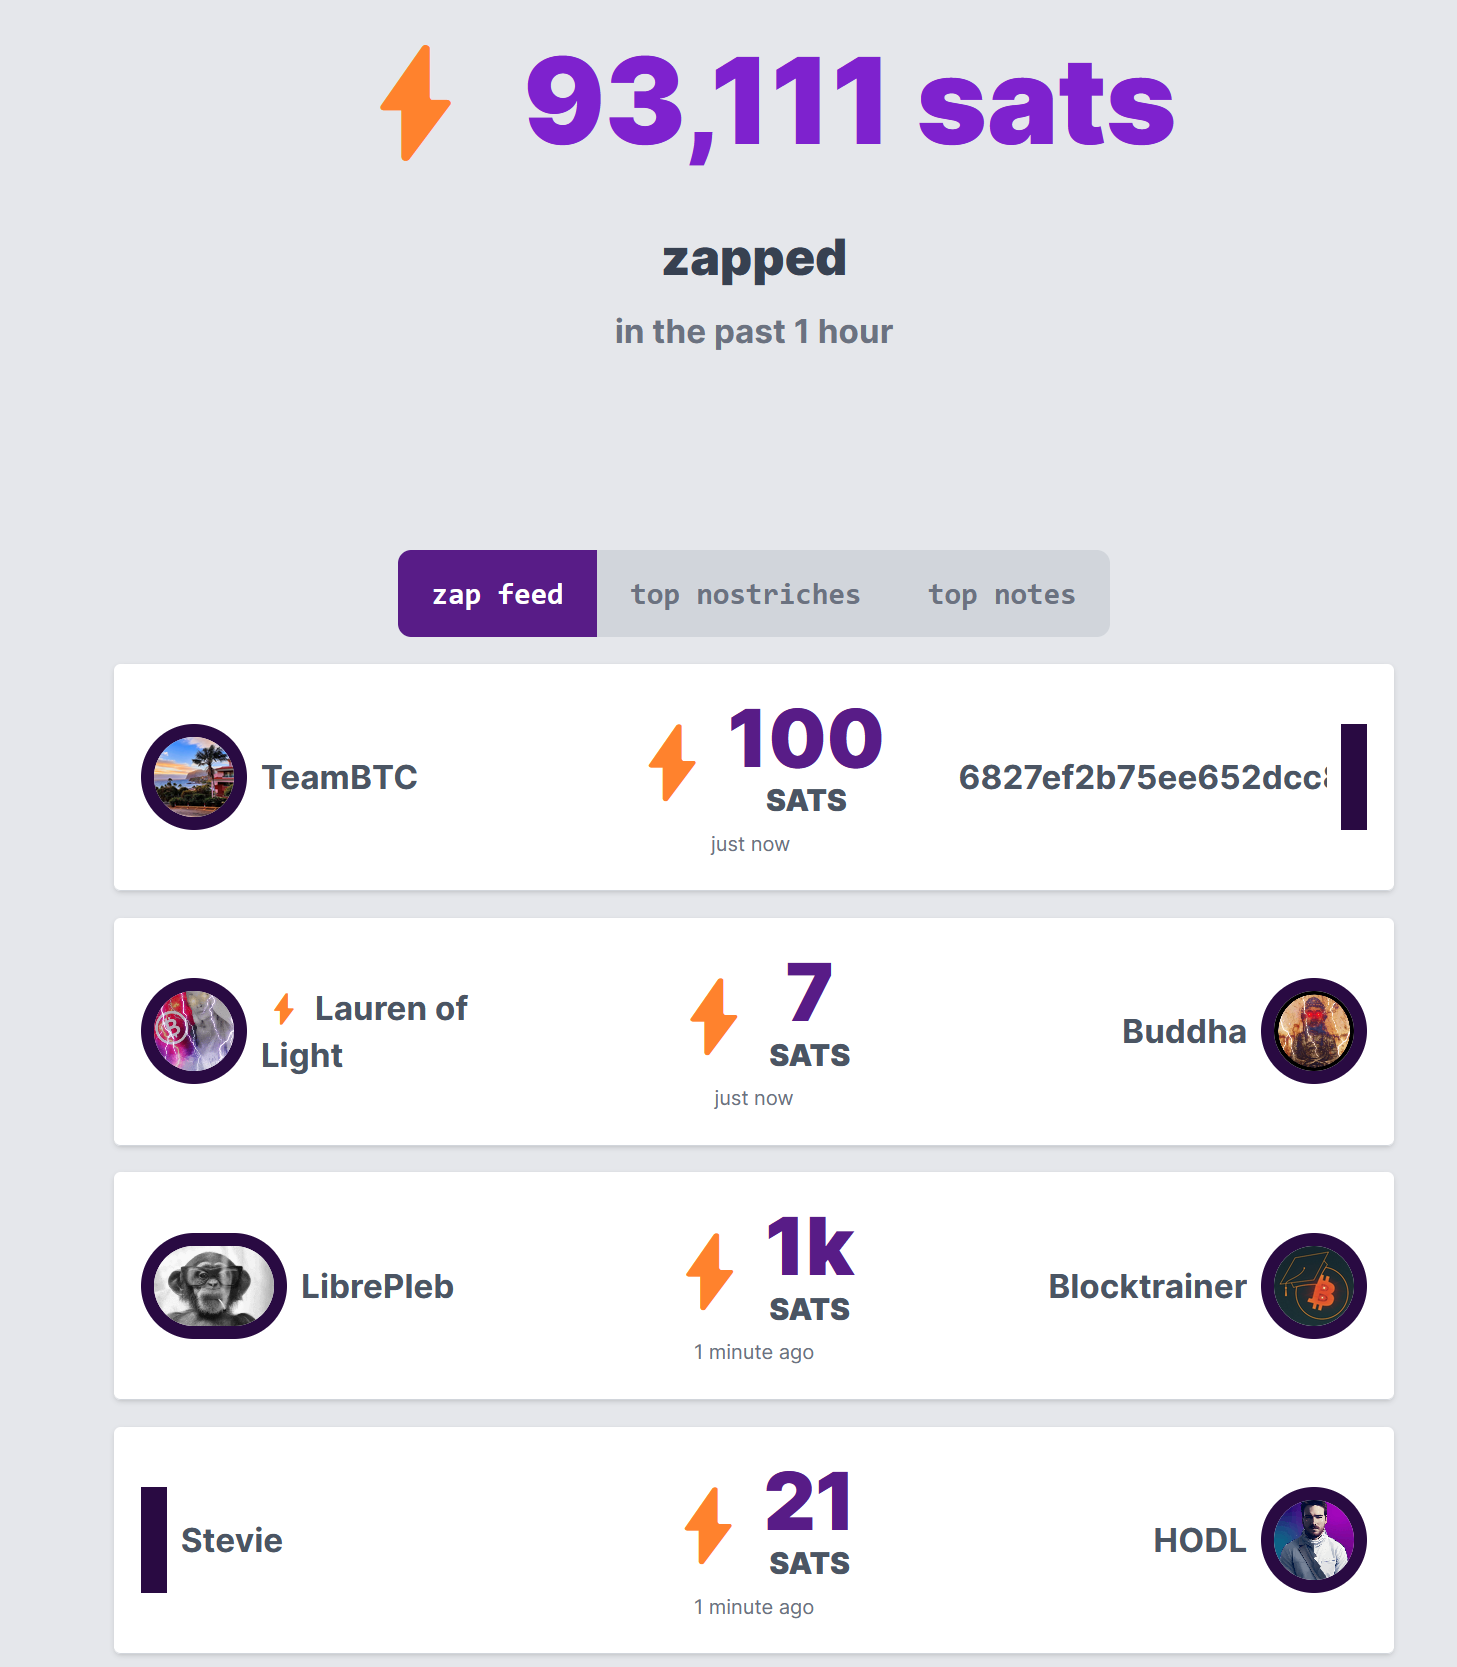
\includegraphics[width=\linewidth*\real{0.5}]{nostrzaps}
  \caption{Within weeks of launch thousands of people are pinging micropayments to one another}
  \label{fig:nostrzaps}
\end{figure}


\subsection{BOLT12 and recurring payments}
\href{https://bolt12.org/}{BOLT12} is a new and developing 'standard' which simplifies and extends the capability of the network for recurring payments, but can negotiate single payments too. The example keyring QR code seen in Figure \ref{fig:bolt12keyring} can be scanned to send single or recurring payments securely and anonymously to the holder.
\begin{figure}
  \centering
    \includegraphics[width=\linewidth*\real{0.5}]{bolt12keyring}
  \caption{\href{https://twitter.com/SeedMint21/status/1518934554840600579}{A key fob with a Bolt12 QR code}}
  \label{fig:bolt12keyring}
\end{figure}
%\subsubsection{Physical Cards}
%\href{https://www.coincorner.com/theboltcard}{Coincorner Bolt card} is an NFC enabled LNURL lightning source which allows tap to pay at lightning enabled vendors. \href{https://www.coindebit.io/}{Coindebit} meanwhile is a VISA card which can be ``charged'' with USD over Lightning. 
\subsection{Cashu and Fedimint}
\subsubsection{Cashu}
Cashu, an implementation of the e-cash mechanism, is an electronic cash system that allows users to hold and transfer digital representations of money on their devices. In this system, e-cash is a piece of electronic data that represents a certain amount of money, such as satoshis in the case of Bitcoin. Users can send e-cash to others through various encrypted channels like Telegram or email.\par
The concept of e-cash relies on blind signatures, which ensure that transactions cannot be correlated to specific users, providing a high level of privacy. When a user wants to send e-cash, they send the data representing the money to another user. The receiving user then sends the e-cash to a server (or mint) to be recycled. This process ensures that the e-cash cannot be double-spent. However, the server cannot correlate the incoming e-cash to any specific user or transaction.\par
Cashu, as a protocol, enables the implementation of this e-cash mechanism and facilitates interoperability among different Cashu wallets. The system is designed to be private, with no user accounts or wallets associated with any central authority. The e-cash is stored in the user's browser data, and can be backed up using a seed phrase, similar to traditional cryptocurrency wallets.\par
In its current state, Cashu is in its early stages of development and is primarily intended for experimentation. However, it has the potential to enable a wide range of applications, such as streaming services, where users could pay for content on a per-use basis without the need for an account, and without the service provider being able to track their usage. This would allow for greater privacy and flexibility in how people interact with online services.
\subsubsection{Fedimint}
From the \href{https://www.fedi.xyz/blog/introducing-fedi-the-global-bitcoin-adoption-technology}{blog post} on the Fedi App website; Fedimint is:
\begin{itemize}
\item a form of community Bitcoin custody,
\item utilising federations (a byzantine fault tolerant multi-sig wallet technology similar to Blockstream's Liquid network),
\item run collectively by groups of trusted community members we call “guardians”,
\item for and on behalf of their communities,
\item with privacy through Chaumian e-cash,
\item and with close integration with the Lightning Network
\end{itemize}
Obi Nwosu sees Fedimint as the third vital pillar of the Bitcoin ecosystem. If Bitcoin is secure decentralised money, and Lightning is decentralised payments, then he says \href{https://bitcoinmagazine.com/technical/fediment-evolution-of-bitcoin-custody}{Fedimint is decentralised custody} of the Bitcoin asset. The excitement in the community is such that this protocol is included in our metaverse stack later. With Fediment a clade of users within the metaverse would have near perfect transactional privacy within their group inside the metaverse \cite{chaum1985security}. This could be a potentially huge group of users, and could include AI actors in the scene. Transactions with the outside world could be through lightning as already planned.
\begin{comment}
\subsection{LNURL-auth}
\href{https://lightninglogin.live/learn}{What is LNURL-auth?}
\textit{``LNURL-auth is a generic authentication protocol. It authenticates the user using digital signatures, which means that the user needs to have a public-private key pair. Thanks to the rising popularity of lightning wallets, more and more users are in possession of and have easy access to such keys. Consequently, users are identified by their public keys, nothing else. The protocol does not require any other identifying information such as passwords, emails, usernames, or similar.''}\par
\textbf{\href{https://github.com/fiatjaf/lnurl-rfc/blob/legacy/lnurl-auth.md}{LNURL-auth} may be able to service all of our user management via LNBits}.
\end{comment}
\subsection{LNBits}
LNBits is an open source, extensible, Lightning `source' management suite. It is self hosted, and can connect to a variety of Lightning wallets, further abstracting the liquidity to provide additional functionality to network users. Remember that all of these tools run without a third party, on a £200 setup, hosted at home or within a business. The best way to explore this is to describe \textit{some} of the plugins. 
\begin{itemize}
\item ``\href{https://github.com/lnbits/lnbits-legend#lnbits-v03-beta-free-and-open-source-lightning-network-walletaccounts-system}{Accounts System}; Create multiple accounts/wallets. Run for yourself, friends/family, or the whole world!''
\item \href{https://github.com/lnbits/lnbits-legend/tree/quart/lnbits/extensions/events#events}{Events plugin} allows QR code tickets to be created for an event, and for payments to be taken for the tickets.
\item \href{https://github.com/lnbits/lnbits-legend/tree/quart/lnbits/extensions/jukebox#jukebox}{Jukebox} creates a Spotify based jukebox which can be deployed online or in physical locations.
\item \href{https://github.com/lnbits/lnbits-legend/tree/quart/lnbits/extensions/livestream#dj-livestream}{Livestream} provides an interface for online live DJ sets to receive real-time Lightning tips, which can be split automatically in real-time with the music producer.
\item \href{https://github.com/lnbits/lnbits-legend/tree/quart/lnbits/extensions/tpos#tpos}{TPoS}, \href{https://github.com/arcbtc/LNURLPoS#lnurlpos}{LNURLPoS} \& \href{https://github.com/lnbits/lnbits-legend/tree/quart/lnbits/extensions/watchonly#watch-only-wallet}{OfflineShop} support online \href{https://rapaygo.com/}{and offline} point of sale (Figure \ref{fig:LnBitsPoS}).
\item \href{https://github.com/lnbits/lnbits-legend/tree/quart/lnbits/extensions/paywall#paywall}{Paywall} creates web access control for content. 
\item \href{https://github.com/LightningTipBot/LightningTipBot#lightningtipbot-}{LightningTipBot} is a custodial Lightning wallet and tip handling bot within the popular on Telegram instant messenger service.
\end{itemize}
\begin{figure}
  \centering
    \includegraphics[width=\linewidth*\real{0.8}]{LnBitsPoS}
  \caption{Two of the many \href{https://rapaygo.com/}{prebuilt} and \href{https://github.com/arcbtc/LNURLPoS}{kit} options for Lightning `point of sale'}
  \label{fig:LnBitsPoS}
\end{figure}
Together these plugins are incredibly useful primitives which are likely to be translatable to a multi party collaborative mixed reality application. A proposal for building a more specific plugin along these lines is detailed later.\par
\textbf{LnBits is capable of backing every object in a metaverse scene as an economic actor, with a key which is compatible with Nostr. This makes it the best choice and it will likely form the core of the proposed metaverse stack.}
\begin{comment}
\subsection{Cashu chaumian mint}
\href{https://github.com/cashubtc/cashu}{Cashu} is a wallet and mint for Bitcoin Lightning that utilizes the Chaumian Ecash implementation, based on David Wagner's variant of Chaumian blinding. It uses token logic similar to minicash and implements a Blind Diffie-Hellman Key Exchange scheme. The database mechanics and the Lightning backend are borrowed from LNbits. With full support for Bitcoin Lightning, Cashu offers a standalone command-line interface wallet and mint server, as well as a mint library that can be included in other Python projects. It supports both PostgreSQL and SQLite databases and includes built-in Tor for hiding IPs during wallet and mint interactions. Additionally, Cashu has a multimint wallet for tokens from different mints and allows you to send tokens to nostr pubkeys.\par
It is possible that thanks to the nostr and lightning integrations we can use this system across our federated metaverse instances to pass fungible `objects' between worlds while maintaining ownership both within and outside of the immersive context. This is an incredibly powerful idea but the security and custody implications are somewhat unclear as the idea is very new.\par 
There is already a \href{https://cashu-wallet.vercel.app/}{promising web interface} to such mints \href{https://bitbucket.org/gandlaf21/cashu-wallet}{in development}.

%\subsection{Etleneum}
%Etleneum is a centralised smart contract platform built around Lightning invoices. It is most notable as a sign of things to come. There are \href{https://etleneum.com/#/contracts}{many small contracts} available to try on the site, such as a \href{https://etleneum.com/#/contract/c8w0c13v75}{simple market} for moving value between lightning and Bitcoin layer 1, or this \href{https://simple-auction.etleneum.com/}{simple auction}.  Contracts are able to operate on data drawn from the wider web, and automatically send and receive lightning payments based on conditional states. It should be viewed as an experiment which allows tinkering in smart contracts, and therefore potentially useful for the software proposed in the final section. There are \href{https://notgeld.medium.com/lightning-network-computation-layer-27c7ba81a214}{suggestions} that this approach might (with some work) allow layer 3 computation more like Ethereum etc.
\subsection{Message passing}
It is possible to pass data alongside lightning payments, routing messages between parties across the global network. This means that a host of other applications can inherit the privacy and censorship resistance of the Lightning network. First amongst these has been simple message passing and group messenger clients such as Sphinx, Juggernaut, Impervious messenger, and RGB Lightning chat. To be clear, this is considered by some to be a misappropriation of the function of the network, and pretty silly given the number of end to end encrypted chat clients available. One more developed use case has been demonstrated by the Impervious development team; they use the message passing capability to negotiate a virtual private network between two parties, using open source software. This allows a secure side channel between internet IP addresses to be opened without a trusted third party. This in itself is a much sought after function of privacy minded networking, and the basis for much of their Impervious browser feature set. 
\end{comment}
\subsection{Daric}
Lightning isn't the only solution to layer 2, as evidenced by Daric \cite{mirzaei2022daric}. This is a complex and technical proposal which claims to improve upon Lightning.
\section{Liquid federation (layer 2)}
Liquid is an implementation on Blockstream \href{https://elementsproject.org/}{Elements}, and is itself part of the open source development contribution of Blockstream, the company started by Adam Back (of hashcash fame) and nearly a dozen other early cypherpunks and luminaries.\par 
The Liquid side chain network, and it's own attendant Lightning layer 2, is a fork of Bitcoin with different network parameters. In liquid the user of the network `pegs' into the Bitcoin network, swapping tokens out from BTC to L-BTC (this can of course mean very small subunits of 1 Bitcoin). Once tokens have been `locked' and swapped to Liquid the different network parameters used in the fork allow a different trust/performance trade-off. Liquid is fast on the L1 chain, cheaper to use at this time, and more private. The consensus achieved on this side chain network is faster because it is a far smaller group of node operators. The next block to be written to the side chain is chosen by a node operated by a member of a federation of dozens of major contributors to the Bitcoin technology space. These `trusted' nodes all check one another's security and network operations, meaning that the network is as secure as the aggregate of the trust placed in half of the membership at any one time. There are
\href{https://bitcoinmagazine.com/business/bitcoin-liquid-network-gains-six-new-federation-members}{still dozens} of major companies, development teams, and individual actors, with significant reputational investment.\par
``Federation members contribute to the Liquid Network's security, gain voting rights in the board election and membership process, and provide valuable input on the development of new features. Members also benefit from the ability to perform a peg-out without a third party, allowing their users to convert between L-BTC and BTC seamlessly within their platform.''\par
Crucially for our purposes here Liquid allows tokenised asset transfer. Anyone \href{https://docs.blockstream.com/liquid/developer-guide/developer-guide-index.html#issued-assets}{can issue} an asset on Liquid. Such transfers of assets may be orders of magnitude cheaper than on chain Bitcoin transactions, but still potentially orders of magnitude more expensive than a simple Lightning transaction of value on the Bitcoin network. \par 
Blockstream plan to add arbitrary (user generated) token support to their `Core Lightning' implementation at some point. This would be a very strong choice for specific use cases within an economically enabled metaverse application. When participants wish to `cash out' of the Liquid network they must do this through one of the federation members who activate the other side of the `two-way peg', dispensing the equivalent amount of Bitcoin. This is transparently handled through Blockstream's ``green wallet''.\par
All of this has the advantage of a far lower energy footprint compared to the main chain, but it's not quite ready with a full suite of affordances. \par
The Liquid network is being used as the underlying asset for a novel new global financial product. El Salvador are working with Blockstream to issue a nation state backed bond. 
\section{Bitcoin Layer 3}
Increasingly important features of modern blockchain implementations are programmability through smart contracts, and issuance of arbitrary tokens. Assigning a transaction to represent another thing like an economic unit, energy unit, or real world object, and operating on those abstractions within the chain logic. Chief among these use cases are stablecoins such as Tether, which are pegged to national currencies and described in the next section. Bitcoin has always supported very limited contracts called scripts, and stablecoin issuance has existed in Bitcoin since 
\href{https://www.omnilayer.org/}{Omni Layer}. Omni was the first issuer of Tether, but more recently these important features have passed to other layer one chains. This year is likely to see the \href{https://www.hiro.so/blog/bitcoin-ecosystem-a-guide-to-programming-languages-for-bitcoin-smart-contracts}{resurgence of this capability} on Bitcoin, which of course benefits from a better security model. Once again, there is a stong assertion by some that \href{https://lists.linuxfoundation.org/pipermail/bitcoin-dev/2022-April/020227.html}{this isn't even possible}. The debate is complex and unresolved.\par 
In order to properly understand the use of Bitcoin based technologies in metaverse applications it is necessary to examine what these newer `layer 3' ideas might bring. 
\subsection{LNP/BP and RGB}
\href{https://giacomozucco.com/layers-before-bitcoin}{LNP/BP} is a non profit standards organisation in Switzerland which contributes to open source development of Bitcoin layer 3 solutions into the Lightning protocol, and Bitcoin protocol (LNP/BP). One of the core product developments within their work is the \href{https://www.rgb.tech/}{`RGB' protocol}, which is somewhat of a meaningless name, evolved from ``coloured coins'' which were an early tokenised asset system on the Bitcoin network. RGB represents red, green, and blue. The proposal is built upon research by \href{https://petertodd.org/2016/commitments-and-single-use-seals}{Todd} and \href{https://giacomozucco.com/#intro}{Zucco}. RGB is regarded as arcane Bitcoin technology, even within the already rarefied Bitcoin developer communities. Zucco provides the \href{https://bitcoinmagazine.com/culture/video-interview-giacomo-zucco-rgb-tokens-built-bitcoin}{following explanation}: \par
\textit{``When I want to send you a bitcoin, I will sign the transaction, I will give the transaction only to you, you will be the only one verifying, and then we’ll take a commitment to this transaction and that I will give only the commitment to miners. Miners will basically build a blockchain of commitments, but without the actual validation part. That will be only left to you. And when you want to send the assets to somebody else, you will pass your signature, plus my signature, plus the previous signature, and so on.''}\par
This is non-intuitive explanation of Todds `single-use-seals', applied to Bitcoin, with the purpose of underpinning arbitrary asset transfer secured by the Bitcoin network. In this model the transacting parties are the exclusive holders of the information about what the object they are transferring actually represents. This primitive can (and has) been expanded by the LNP/BP group into a concept called `client side validation'. 
It's appropriate to explain this concept several times from different perspectives, because this is potentially a profoundly useful technology for metaverse applications.\par
\begin{itemize}
\item A promise is made to spend a multi output transaction in the future. This establishes the RGB relationships between the parties.
\item One of the pubkeys to be spent to is known by both parties.
\item The second output is unknown and is a combination of the hash of the state, and schema, from the operation which has been performed.
\item When the UTXO is spent the second spends pubkey can be processed against the shared data blob to validate the shared state in a two party consensus  (sort this out, it's nonsense).
\item This is now tethered to the main chain. Some tokens from the issuance have gone to the recipiant, and the remainder have gone back to the issuer. More tokens can be issued in the same way from this pool. 
\item A token schema in the blob will show the agreed issuance and the history back to the genesis for the token holder. 
\item The data blob contains the schema which is the key to RGB functions and the bulk of the work and innovation. 
\item Each issuance must be verified on chain by the receiving party. 
\end{itemize} 
This leverages the single-use-seal concept to add in smart contracts, and more advanced concepts to Bitcoin. Crucially, this is not conceptually the same as the highly expressive `layer one' chains which offer this functionality within their chain logic. In those systems there is a globally available shared consensus of `state'. In the LNP/BP technologies the state data is owned, controlled, and stored by the transacting parties. Bitcoin provides the crytographic external proof of a state change in the event of a proof being required. This is an elegant solution in that it takes up virtually no space on the blockchain, is private by design, and is extensible to layer 2 protocols like Lightning.\par
This expanding ecosystem of client side verified proposals is as follows:
\begin{itemize}
\item RGB smart contracts
\item RGB assets are fungible tokens on Bitcoin L1 and L2, and non fungible Bitcoin L1 (and somewhat on L2).
\item Bifrost is an \href{https://github.com/LNP-BP/presentations/blob/master/Presentation slides/Bifrost.pdf}{extension} to the Lightning protocol, with it's own Rust based node implementation, and backwards compatibility with other nodes in the network. This means it can transparently participate in normal Lightning routing behaviour with other peers. Crucially however it can also negotiate passing the additional data for token transfer between two or more contiguous Bifrost enabled parties. This can be considered an additional network liquidity problem on top of Lightning, and is the essence of the ``Layer 3'' moniker associated with LNP/BP. It will require a great number of such nodes to successfully launch token transfer on Lightning. As a byproduct of it's more `protocol' minded design decisions Bifrost can also act as a generic peer-to-peer data network, enabling features like Storm file storage and Prometheus.
\item \href{https://www.aluvm.org/}{AluVM} is a RISC based virtual machine (programmable strictly in assembly) which can execute Turing complete complex logic, but only outputs a boolean result which is compliant with the rest of the client side validation system. In this way a true or false can be returned into Bitcoin based logic, but be arbitrarily complex within the execution by the contract parties.
\item Contractum is the proposed smart contract language which will compile the RGB20 contracts within AluVM (or other client side VMs) to provide accessible layer 3 smart contracts on Bitcoin. It is a very early proposal at this stage.
\item  Internet2: ``Tor/noise-protocol Internet apps based on Lightning secure messaging
\item Storm is a lightly specified escrow-based bitcoin data storage layer compliant with Lightning through Bifrost.
\item Prometheus is a lightly specified multiparty high-load computing framework.
\end{itemize}
Really, any compute problem can be considered applicable to client side validation. In simplest terms a conventional computational problem is solved, and the cryptographically verifiable proof of this action, is made available to the stakeholders, on the Bitcoin ledger.\par 
Less prosaically, at this stage of the project the more imminent proposed affordances of LNP/BP are described in `schema' \href{https://github.com/LNP-BP/LNPBPs}{on the project github}. The most interesting to the technically minded layperson are:
\begin{itemize}
\item \href{https://github.com/LNP-BP/LNPBPs/blob/master/lnpbp-0020.md}{RGB20} fungible assets. This could be stablecoins like dollar or pounds representation. Bitfinex exchange \href{https://github.com/RGB-Tools/rgb-lightning-sample}{have code} which already works with RGB to transmit Tether stablecoins on testnet. This is a huge application area for Bitcoin, and similar to Omni, which will also be covered next.
\item \href{https://github.com/LNP-BP/LNPBPs/blob/master/lnpbp-0021.md}{RGB21} for nonfungible tokens and ownership rights. In principle BiFrost allows these to be transferred over a the Lightning network, significantly lowering the barrier to entry for this whole technology. DIBA \href{https://diba.io/}{have this technology working} on testnet.
\item \href{https://github.com/LNP-BP/LNPBPs/issues/29}{RGB22} may provide a route to identity proofs. This is covered in detail later.
\end{itemize}
Federico Tenga is CEO of `Chainside' and an educator and consultant in the space. He has written an up-to-date \href{https://medium.com/@FedericoTenga/understanding-rgb-protocol-7dc7819d3059}{``primer''}, which is still extremely complex for the uninitiated, but does capture how the RGB token transfer system works. That medium article also touches on Taro, which is next.
\subsection{Taro}
Taro is an very new \href{https://lightning.engineering/posts/2022-4-5-taro-launch/}{initiative by Lightning Labs} to allow assets to transmit on the Lightning network. It is more similar to RGB above than Omnibolt below. They say: \textit{``Taro enables bitcoin to serve as a protocol of value by allowing app developers to integrate assets alongside BTC in apps both on-chain and over Lightning. This expands the reach of Lightning Network as a whole, bringing more users to the network who will drive more volume and liquidity in bitcoin, and allowing people to easily transfer fiat for bitcoin in their apps. More network volume means more routing fees for node operators, who will see the benefits of a multi-asset Lightning Network without needing to support any additional assets.''}\par
The project has clearly been \href{https://github.com/roasbeef/bips/tree/bip-taro}{under development} by the lead developer at Lightning Labs for some years and seems both \href{https://lightninglabs.substack.com/p/bitcoinizing-the-dollar-and-the-world?s=r}{capable} and mature, though they are obviously following the model of `co-opting' open source ideas (from RGB) to garner venture capital funding. They \href{https://github.com/bitcoin/bips/pull/1298/commits/4daba8c373c777defb48136795382803c137502c}{credit RGB} in the github. More will doubtless be added to this section and it seems a contender for our metaverse purposes, being less broadly ambitious than RGB upon which it's based, but perhaps more focused and implemented. The key feature of Taro seems to be that only the first and last hop in a multi-hop lightning transaction need to support Taro, because of external data validation databases called ``universes''. This is an advance on the RGB proposal. 
The technical specs are now on the \href{https://docs.lightning.engineering/the-lightning-network/taro}{lightning labs web pages}, and \href{https://lightning.engineering/posts/2022-9-28-taro-launch/}{code has been released}. The beta programme uses testnet. There are concerns that large amounts of synthetic dollars on the protocol could be used to create `incentive' for one Bitcoin hard fork or another, under the control of Tether. 
\begin{comment}
\subsection{Slashpay}
Slashpay is a very promising and recent product, and part of a suite of interlinked (Bitcoin compatible) layer 3 ideas. It is \textit{not} a blockchain technology, but it is highly intersectional with Bitcoin. The Synonym suite is advocating what they call the `Atomic Economy', an overarching abstraction of any of the technologies in the space into a single cryptographic key pair, with all the other products nested under it. The suite will be selected and unpacked for metaverse purposes later, but for this section the Slashpay product integrates as a layer three idea, building upon lightning. \par
Slashpay gathers all of the available Lightning invoice and QR code `standards' under an abstracted metastandard with it's own key pair. This allows a negotiation between party and counterparty in code, which settles on agreeable standards for the value transfer. The Slashpay mediation metadata is embedded in the top level Slashtag QR code. Within the Slashpay element of the data is a priority list for the exchange, which can be changed by the user according to their capability and preferences.\par 
The code to support this is in a early stage. There is a minimum viable product which can negotiate between online Lightning nodes. The advantage of the Slashpay method, and the thing that puts it in the layer 3 section, is that in the event of a failed Lightning payment (for whatever reason), the software can then default to the next payment method in it's negotiated list. This would most likely be another (different) Lightning attempt, or a Bitcoin main chain transaction.\par
This technical ecosystem uses a `distributed hash table' to hold and negotiate keys, stored using Hypercore, another external project based on Bittorrent. This is the \href{https://hypercore-protocol.org/protocol/#hyperswarm}{`Hyperswarm DHT'}, which has potential uses elsewhere in the collaborative mixed reality use cases.\par
There is clearly additional complexity in setting this system up, but once in place it might provide a unified way to scale capability under the evolving standard.  
\end{comment}
\subsection{Spacechains}
Spacechains is a \href{https://medium.com/@RubenSomsen/21-million-bitcoins-to-rule-all-sidechains-the-perpetual-one-way-peg-96cb2f8ac302}{proposal} by Ruben Somsen. It is a way to provide the functionality of any conceivable blockchain, by making it a sidechain to Bitcoin. \par
Like RGB described earlier it's a single use seal, but which can be closed by the highest bidder.\par
In a spacechain the Bitcoin tokens are destroyed in order to provably create the new spacechains tokens at a 1:1 value. These new tokens only have worth moving forward within the new chain ecosystem they represent, as they cannot be changed back. They nontheless have the same security guarantees as the bticoin main chain, though with a radically reduced ecological footprint (x1000?), and higher performance. Each `block' in the new chain is a single bitcoin transaction. The high level features are:\par
\begin{itemize}
\item Outsource mining to BTC with only a single tx per block on the main chain.
\item One way peg, Bitcoin is burnt to create spacechain tokens.
\item Allows permissionless chain creation, without a speculative asset.
\item Fee bidding BMM is space efficient and incentive compatible. Miners just take the highest fees as normal.
\item Paul Sztorc raised the idea
\item It's best with a soft fork but possible without
\end{itemize}
The concept is \href{https://vimeo.com/703246895/d89aba6e56}{explained fully} in a recent presentation at Advancing Bitcoin conference.\par 
Developer Fiatjaf, a stalwart of the the lightning developer community has a basic Spacechains based \href{https://github.com/nbd-wtf/soma}{asset trading system} which can be run already called Soma, though it is limited to Signet, one of the local bitcoin testnets, modified with AnyPrevOut described elsewhere in the book.

%\subsection{Drivechain}
%\lipsum[50]
%\subsection{Softchains}
%\lipsum[50] 
\subsection{Statechains, drivechain, softchains} 
There are many \href{https://gist.github.com/RubenSomsen/96505e99dc061d6af6b757ff74434e70}{proposals for layer 2 scaling solutions} for the bitcoin network. Ruben Somsen \href{https://gist.github.com/RubenSomsen/c9f0a92493e06b0e29acced61ca9f49a}{describes Softchains, Stateschains, and Spacechains}, while  \href{https://www.drivechain.info/literature/index.html}{Drivechain is described} by the author Paul Sztorc on the project web pages and is split across \href{https://github.com/bitcoin/bips/blob/master/bip-0300.mediawiki}{BIP-0300} for drivechain and \href{https://github.com/bitcoin/bips/blob/master/bip-0301.mediawiki}{BIP-0301} for a ``blind merge mining'', a soft fork which it's unlikely to get. They are all hypothetical with the exception of sidechains.  

\begin{comment}}
\section{Other chains and networks}
It's useful to make some `honourable mentions' of other options as this technology is moving so fast. These chains are viewed by some as a kind of triage for ideas which might one day find their way into Bitcoin. This is potentially most true of zk rollups which might eventually migrate from privacy and scaling experiments on \href{https://docs.ethhub.io/ethereum-roadmap/layer-2-scaling/zk-starks/}{other chains} \cite{BenSasson2022}. This list simply isn't very useful in terms of judging other chains, as they rise and fall so fast. To be clear, there is a fundamental \textit{legal} difference between all of the 15,000 or so attempts at layer 1 chains after Bitcoin, in that they are controlled by a subset of people who have an incentive to lie about the usefulness of the technologies they are invested in. This lack of useful decentralisation has been touched on but is dealt with in detail by Microstrategy CEO Michael Saylor in a \href{https://www.youtube.com/watch?v=mC43pZkpTec}{four hour podcast} with Ai researcher Lex Fridman. It's interesting that Saylor (who is a significant educator in the space) views custodial companies holding Bitcoin on behalf of their clients as Bitcoin layer 3. All of this is new enough that virtually all of it is contested by someone. To demonstrate the difference between Bitcoin as a property vs alt coins as `securities in law' it's useful to see the allocations of tokens to seed investors in some of the newer chains in Figure \ref{fig:messariICO}.

\begin{figure}
  \centering
    \includegraphics[width=\linewidth]{messariICO}
  \caption{Allocations given at the beginning of public blockchain, by Messari.}
  \label{fig:messariICO}
\end{figure}

\subsection{Layer 1 chains}
As the market wanes in 2022 the fragility of tokens other than Bitcoin is being exposed. They are suffering brutal losses. Historically tokens spend around 19 weeks in the top tier of tokens before falling away. Each cycle brings and new crop during the bull market and these invariably don't make it through to the next cycle. There are a few which have longevity and name recognition, but mainly because they amassed enough capital during the early days to play a very long, if somewhat pointless game.
\begin{itemize}
\item Monero is a privacy focused coin with a great deal of credible and competent developer attention. It attracts a lot of criticism precisely because it's anonymity by design makes it perfect for nefarious activity such as drugs markets. Privacy advocates in the space say that total unaccountability of money is a `must have' feature and that \href{https://sethforprivacy.com/posts/dispelling-monero-fud/#introduction}{critiques of the chain} are in bad faith. It's actually arguably the best of the alternatives, having a valid use case  in privacy.
\item Solana is a far more centralised layer 1 proposition which uses a few hundred highly performant nodes to achieve high transaction throughput. The consensus algorithm is the novel \href{https://solana.com/solana-whitepaper.pdf}{``proof of history''} system. Development of the technology has been funded and supported by huge venture capital investment, and even though the chain is quite unreliable it seems that the vested interests of the investors can keep interest going. It is cheaper, and more useful than Bitcoin and Ethereum, but lacks longevity and reliability. It could probably be a database. With that said it is well funded, and fun to use. They have \href{https://solana.com/news/solana-mobile-stack-reveal}{announced a mobile stack} and a first foray into making an android mobile phone to leverage it. This would, they say, allow a whole new model of mobile Web3 interaction.
\item Polkadot is much hyped within the ``crosschain'' protocol community. These chains connect the logic of a smart contract on one chain to that of another. In practice, while it is possible that this is useful for distributed finance products, it seems that chains such as DOT might be promising more than the markets actually want or need. Governance of the token is a DAO like model where staking (locking up) the tokens theoretically controls the direction of the product. Crosschain products like this are a \href{https://blog.chainalysis.com/reports/cross-chain-bridge-hacks-2022/}{cybersecurity nightmare}.
%\item Terra is a relatively new \href{https://assets.website-files.com/611153e7af981472d8da199c/618b02d13e938ae1f8ad1e45_Terra_White_paper.pdf}{ecosystem offering} with a stablecoin, and DeFi built in. It is currently in ascendancy (\$15 in a year) and seems to have a stable and useful underpinning, but is far too new to judge with any certainty. There's more on this in the stablecoin section later.
%\item Avalanche AVAX is a newer, `faster' and more eco friendly DeFi ecosystem which promises returns within it's own framework of permissionless money. It is one of the relative success stories of the DeFi narrative. It's unclear what the value proposition, and sustainability of this token actually are.
\item TRON TRX draws extensive criticism for being founded by \href{https://www.theverge.com/c/22947663/justin-sun-tron-cryptocurrency-poloniex}{Justin Sun}. A huge amount of value transacts on TRON, mainly thanks to the Tether stablecoin, and it could be argued that this gives it a genuine use case. It's more likely another house of cards.
\item Tezos is a well established player with an early and somewhat battle tested proof of stake mechanism and distributed governance model. It has attracted many high profile partnerships and sponsors, but is primarily seeking to be a store of value token like bitcoin, which exposes the chain to the ``winner takes all'' landscape of digital money. There are some compelling NFT advocates of the technology, which is certainly `greener' and cheaper to use, but the longevity in such an irrational market is uncertain, because it does not seem to have the network effect and growth velocity. 
\item Algorand's ALGO token purports to be a more modern and useful proof of stake value transfer chain. It is fundamentally similar to Tezos.
\item IOTA is noteworthy, interesting, and established concept, with an edge use case. It is a `distributed ledger of the internet of things', the much hyped and clearly extant ecosystem of edge compute, sensors, smart devices etc. The marketing around IOTA correctly identifies it's positioning and potential within this developing technology ecosystem, but it's primary use case is too nascent and too niche, and the implementation itself has drawn (valid) \href{https://medium.com/@neha/cryptographic-vulnerabilities-in-iota-9a6a9ddc4367}{criticism for amateurish cryptography} and a fundamentally centralised model. The concept remains interesting.
\item VeChain is a long established platform with `significant' industry adoption which still doesn't represent it's market capitalisation, usefulness, or future success. It is the most exposed of all the chains to the untruth that immutable global ledgers, of real world assets, somehow protect from fraudulent behaviour. It's perhaps useful, but mainly in a highly automated industry 4.0 environment, with minimal human interaction. 
\item Cardano foundation ADA is one of the more established players and has been developing methodically and slowly. They have made great strides in successfully enabling a provable proof of stake consensus structure. Proof of stake non-the-less has significant problems in that tokens and therefore control inevitably concentrates over time. There is no proposed solution to this. They have working products and partnerships, but perhaps not as many as the market cap of the ecosystem would suggest. 
\item HBAR claims ``third generation'' blockchain technology, with carbon positive, high speed, distributed applications. There are always tradeoffs bound by physical constraints within distributed computing, and Hedera HBAR has been accused of a cryptographic model which is inherently insecure.
\item EOS is one of the early major successes of the ICO funding model in 2017, and they amassed an enormous war chest of bitcoin which they still hold. The onus is on them to deliver some kind of product, and they have the funds to do so, but they probably won't.
\end{itemize}
%\subsection{Distributed data storage}
%\lipsum
\end{comment}
\subsection{Layer 2}
The only non Bitcoin layer two of note at this time is the recently announced `Base' from Coinbase. It is built on top of Optimism's op stack, which is itself built on Ethereum. Base is intended to offer a secure, low-cost, developer-friendly platform for building decentralized applications on Ethereum L2. The network is also expected to bridge to other L2s and L1s, including Bitcoin.\par
Coinbase's decision to invest in a decentralized layer 2 network without launching a token represents a departure from the current trend of tokenizing everything in the cryptocurrency industry. The move may signal a long-term commitment to creating sustainable value in the ecosystem, rather than seeking short-term gains through token issuance. Coinbase will contribute 20\% of sequencer revenue to fund public goods, and Base is intended to be an open-source project.\par
Base's potential to compete with centralized exchanges such as Binance Smart Chain is a notable aspect of the announcement. While BSC has gained significant traction by offering a cheaper and faster alternative to Ethereum, its ties to Binance create regulatory issues and raise questions about both centralisation and its long-term sustainability. In contrast, Base is intended to be a decentralized network that can be used to build a wide range of applications, without being tied to a specific centralized company.\par
Base also positions itself as the KYC option for real-world assets and securities coming on-chain. While this could create some benefits in terms of compliance and regulatory oversight, it could also limit the potential for decentralized innovation and create new risks for user privacy. There are significant questions and concerns about the project, the fact that it is an open-source initiative and is intended to be a decentralized network (in the end) suggests that Coinbase is taking a long-term view of its role in the blockchain ecosystem.
\section{Risks and mitigations}
Looking across the whole sector, this paragraph from the Bank of International Settlement (BIS) \href{https://www.bis.org/publ/arpdf/ar2022e3.htm}{sums everything up}: \par
\textit{``...it is now becoming clear that crypto and DeFi have deeper structural limitations that prevent them from achieving the levels of efficiency, stability or integrity required for an adequate monetary system. In particular, the crypto universe lacks a nominal anchor, which it tries to import, imperfectly, through stablecoins. It is also prone to fragmentation, and its applications cannot scale without compromising security, as shown by their congestion and exorbitant fees. Activity in this parallel system is, instead, sustained by the influx of speculative coin holders. Finally, there are serious concerns about the role of unregulated intermediaries in the system. As they are deep-seated, these structural shortcomings are unlikely to be amenable to technical fixes alone. This is because they reflect the inherent limitations of a decentralised system built on permissionless blockchains.''}\par
This might seem like reason enough to  stop here and wait for proper digital currency (expanded later), but Bitcoin is here now, is likely unstoppable in, and with mitigations in place might have uses if developed properly. Perhaps surprising the same BIS is \href{https://www.bis.org/press/p221216.htm}{allowing up to 2\%} of bank reserves to be held in crypto assets, including Bitcoin, \href{https://www.bis.org/bcbs/publ/d533.pdf}{according to their June 2022 Basel Committee on Banking Supervision report}, though the BIS chief believe the \href{https://www.bloomberg.com/news/articles/2023-02-22/crypto-has-lost-battle-against-fiat-currency-bis-chief-agustin-carstens-says}{``battle'' against crypto} has already been won following the turmoil described in the next section. \par
Lightning is still considered to be experimental and not completely battle tested. There have been various attacks and a major double spend attack may be possible \cite{https://doi.org/10.48550/arxiv.2208.01908}, but there have been no major problems in the years it's been running with careful design choices and cybersecurity best practice it it likely a production ready component of our planning.
\subsection{Sociopaths \textbf{everywhere}}
In the wake of the \href{https://www.bloomberg.com/opinion/articles/2022-11-14/ftx-s-balance-sheet-was-bad}{rampant crime spree} by Sam Bankman-Freid and his top teams at Alameda research and the Bahamas registered exchange `FTX' the whole industry has suffered, and will continue to suffer, seismic shocks. There is a chance the sector will never recover, and that we have already seen the top of the hype bubble. Fortunately this doesn't diminish our use cases for these technologies, as we were never planning to speculate with the asset, but rather use the network.
\subsection{Digital assets}
For digital assets more generally it is useful to look at the recent \href{https://www.whitehouse.gov/briefing-room/presidential-actions/2022/03/09/executive-order-on-ensuring-responsible-development-of-digital-assets/}{``whole government executive order''} signed by President Biden early in 2022. It was mainly framed in terms of ``responsible innovation, and leadership'' in the new space. The resulting, ``Comprehensive Framework for Responsible Development of Digital Assets'' is a product of multi agency collaboration and can be seen as 9 reports and a summary document, and has been long anticipated. The summary itself is neither particularly comprehensive nor a framework, and mainly serves to identifies high level risks, aspirations, and challenges, and strongly hints toward eventual development of a ``digital dollar'' (CBDC, expanded later). \par
The risks section of the original executive order shows how legislators are framing this, so it's useful to break down here.\par
\begin{itemize}
\item Consumer and business protections. This is likely to pertain to custodians and is much needed. Misselling is rife. Security presents a challenge.  
\item Systemic risk, and market integrity are a concern. The legislators clearly worry about contagion risks from the sector.
\item Illicit finance (criminality and sanction busting etc) are a concern, but not particularly front and centre\cite{moser2013inquiry}. Criminality in 2021 was a mere 0.15\% of transactions according to Chainalysis, but this number varies year to year. There are claims that Iran have begun official overseas buying with cryptocurrencies, but again, the \href{https://finbold.com/iran-makes-the-first-ever-import-of-goods-using-cryptocurrency-worth-millions/}{numbers are small}. One of the better sections of the work is the US treasury department's recently published `National Risk Assessments for Money Laundering, Terrorist Financing, and Proliferation Financing'. This is a comprehensive report and speaks to careful research across the space. It is broken into \href{https://home.treasury.gov/news/press-releases/jy0619}{three parts}. Perhaps surprisingly, while they do see activity in these areas, they do not rate the risk as very significant. Cash remains the main problem for illicit funding. There is some talk that the nature of public blockchain analysis allows greater oversight of these tools and that this is to the advantage of government and civil enforcement agencies.
\item Highlighting the need for international coordination suggests they are mindful of jurisdictional arbitrage. 
The partial regulatory capture of these technologies, where activity flows to globally more lenient legislative regimes, continues to be a concern. Many of the centralised exchanges for instance are located in tax havens such as Malta. As the world catches up with these products it is likely that this will be smoothed out.
\item Climate goals, diversity, equality and inclusion are mentioned. It seems that the ``environment'' aspect of ESG is more important then ``social'' and ``governance'' at this time.
\item Privacy and human rights are mentioned.
\item Energy policy is highlighted, including grid management and reliability, energy efficiency incentives and standards, and sources of energy supply.
\end{itemize}
The \href{https://www.whitehouse.gov/briefing-room/statements-releases/2022/09/16/fact-sheet-white-house-releases-first-ever-comprehensive-framework-for-responsible-development-of-digital-assets/}{latest summary report} resulting from the above guidance actually adds little tangible meat to the bones. This possibly reflects the complexity of these issues. The recommendations seem to be broadly as follows, and are really a copy/paste of the executive order.
\begin{itemize}
\item Carry on doing research into central bank digital currencies, but there's no particular rush.
\item Support development of better instant payment methods both at home and globally. 
\item Ensure consumer and systemic protections.
\item More monitoring, civil and criminal prosecutions.
\item Issue more rules and clarity in response to risks (this is actually likely net positive as rules are currently unclear).
\item Improve global reporting on users (KYC/AML).
\end{itemize}
The government rhetoric to date in the USA can be seen to be converging on an understanding of the technology, at different rates in different parts of government. One thing that seems to shine through is their own perception of their global leadership on legislation on these matters. They seems to assume that what they decide will guide the world, and this may be true through their KYC/AML pressures.\par
A recent proposed \href{https://bitcoinmagazine.com/business/heres-whats-in-senator-lummis-bitcoin-bill}{bi-partisan bill in the USA} will likely help inform global law, though it is unlikely to pass itself. It encourages the use of Bitcoin as a medium of exchange by applying a tax exemption on transactions of less than \$200. The issue of whether an asset is a commodity (a raw material thing) or a security (a promise) is left to a couple of major government agencies to unpick, with corresponding reporting requirements. Crucially for this book these nascent bills all regard both Bitcoin and Ethereum as sufficiently decentralised to \href{https://www.coincenter.org/a-new-senate-bill-focuses-on-cryptocurrency-exchanges-heres-what-developers-and-users-should-keep-an-eye-on/}{qualify as commodities}, meaning they would enjoy more lenient oversight. Far more likely to pass is the \href{https://www.agriculture.senate.gov/imo/media/doc/crypto_one-pager1.pdf}{proposed DCCPA bill} which has senior lawmaker support and would see commodities in the space regulated in such a way that trading of it could be halted in the USA. In this line of policy, exchanges will be required to do far more reporting, and would be penalised for trading against their customers. DOAs and DeFi are the big potential losers. In a maddening twist the Office of Government Ethics in the USA has banned anyone who owns digital assets from working on the legislation. This is an exceptional move and likely to result in poorly crafted laws in the first instance.\par
The most recent and troubling example is the US ban on any Ethereum assets which have been through a ``mixer service'' \href{https://www.coincenter.org/u-s-treasury-sanction-of-privacy-tools-places-sweeping-restrictions-on-all-americans/}{that obfuscates history}. This is a huge constraint on the code and smart contract itself, not just sanctions against individuals. It has \href{https://hoffmang9.github.io/free-speech/the-history-code-is-free-speech.html}{`free speech'} and constitutional implications \cite{anderson2002free}. More such actions and \href{https://www.dw.com/en/dutch-investigators-say-developer-of-tornado-cash-arrested/a-62793823}{arrests of developers} are feared. It has led to Circle (who issue the USDC stablecoin) blacklisting every \href{https://home.treasury.gov/policy-issues/financial-sanctions/recent-actions/20220808}{address sanctioned by the US government}. Centrally issued digital assets are obviously neither uncensorable nor permissionless. This intersects (again) with the whole question of what decentralisation means and how effective it can be in it's stated goal of circumventing global policies.
\subsection{Bitcoin specifically}
\noindent In addition it's useful for this document to focus more on the technical challenges to the Bitcoin network.\par
\begin{itemize}
\item The block reward is reduced every 4 years (epochs). This means a portion of the mining reward is trending to zero, and nobody knows what effect this will have on the incentives for \href{https://www.truthcoin.info/blog/security-budget-ii-mm/}{securing the network} through proof of work \cite{carlsten2016instability}. It is increasingly \href{https://cryptostackers.substack.com/p/bitcoin-is-not-a-store-of-value?sd=pf&s=r}{being discussed} as the major eventual problem for the network.
\item Stablecoins are a vital transitional technology (described later) but do not meaningfully exist yet on the Bitcoin network. This may change.
\item Bitcoin lacks privacy by design. All transactions are publicly viewable. This is a major drag to the concept of BTC as a money. Upgrade of the network is possible, and has indeed been achieved for a Bitcoin fork called Litecoin \cite{fuchsbauer2019aggregate}. 
\item The Lightning network (described later) has terrible UX design at this time. 
\item The basic `usability' of the network is still poor in the main. Any problems which users experience demand a steep learning curve and risk loss of funds. There is obviously no technical support number people can call. 
\item Only around one billion unspent transactions can be generated a year on the network. This means that it might become impossible for everyone on the planet to have their own Bitcoin address (with it's associated underpinning UTXO).  
\item Chip manufacture is concentrated in only a few companies and countries, as identified by \href{https://www.btcpolicy.org/authors/matthew-pines}{Matthew Pines}. %He also identifies the \href{https://www.btcpolicy.org/#Research}{these points}.
\item Potential constraints on monetary policy flexibility.
\item Future protocol changes.
\item Unanticipated effects on the domestic and international energy system.
\item Vulnerability to adversary attacks are \href{https://braiins.com/blog/bitcoin-mining-attacks-explained}{widely studied}\cite{apostolaki2016hijacking, apostolaki2017hijacking, johnson2014game, stinner2022proof}, and still pretty much completely speculative because of the complex nature of the attack surface.
\item Mining tends toward economy of scale concentration. Many are already on their \href{https://bitcoinfibre.org/}{own specialised network} to connect to one another.
\item Future hard forks. There will doubtless be pressure to fork the code to add inflation, or ESG mitigations, or to fix the UNIX clock issue in 2106. Each fork is a risk.
\item Other unknown, unanticipated risks given Bitcoin’s limited 13-year history.
\item There is a ``non-zero'' chance that Bitcoin is a complex government intelligence agency construct, \href{https://en.wikipedia.org/wiki/Crypto_AG}{much like Crpto AG was} toward the end of the last century \cite{dymydiuk2020rubicon}. 
\end{itemize} 


%\subsection{Crime and santion busting}
%
